% Options for packages loaded elsewhere
% Options for packages loaded elsewhere
\PassOptionsToPackage{unicode}{hyperref}
\PassOptionsToPackage{hyphens}{url}
\PassOptionsToPackage{dvipsnames,svgnames,x11names}{xcolor}
%
\documentclass[
  12pt,
  letterpaper,
]{scrartcl}
\usepackage{xcolor}
\usepackage[top=2.5cm,bottom=2.5cm,left=2.5cm,right=2.5cm]{geometry}
\usepackage{amsmath,amssymb}
\setcounter{secnumdepth}{-\maxdimen} % remove section numbering
\usepackage{iftex}
\ifPDFTeX
  \usepackage[T1]{fontenc}
  \usepackage[utf8]{inputenc}
  \usepackage{textcomp} % provide euro and other symbols
\else % if luatex or xetex
  \usepackage{unicode-math} % this also loads fontspec
  \defaultfontfeatures{Scale=MatchLowercase}
  \defaultfontfeatures[\rmfamily]{Ligatures=TeX,Scale=1}
\fi
\usepackage{lmodern}
\ifPDFTeX\else
  % xetex/luatex font selection
\fi
% Use upquote if available, for straight quotes in verbatim environments
\IfFileExists{upquote.sty}{\usepackage{upquote}}{}
\IfFileExists{microtype.sty}{% use microtype if available
  \usepackage[]{microtype}
  \UseMicrotypeSet[protrusion]{basicmath} % disable protrusion for tt fonts
}{}
\usepackage{setspace}
\makeatletter
\@ifundefined{KOMAClassName}{% if non-KOMA class
  \IfFileExists{parskip.sty}{%
    \usepackage{parskip}
  }{% else
    \setlength{\parindent}{0pt}
    \setlength{\parskip}{6pt plus 2pt minus 1pt}}
}{% if KOMA class
  \KOMAoptions{parskip=half}}
\makeatother
% Make \paragraph and \subparagraph free-standing
\makeatletter
\ifx\paragraph\undefined\else
  \let\oldparagraph\paragraph
  \renewcommand{\paragraph}{
    \@ifstar
      \xxxParagraphStar
      \xxxParagraphNoStar
  }
  \newcommand{\xxxParagraphStar}[1]{\oldparagraph*{#1}\mbox{}}
  \newcommand{\xxxParagraphNoStar}[1]{\oldparagraph{#1}\mbox{}}
\fi
\ifx\subparagraph\undefined\else
  \let\oldsubparagraph\subparagraph
  \renewcommand{\subparagraph}{
    \@ifstar
      \xxxSubParagraphStar
      \xxxSubParagraphNoStar
  }
  \newcommand{\xxxSubParagraphStar}[1]{\oldsubparagraph*{#1}\mbox{}}
  \newcommand{\xxxSubParagraphNoStar}[1]{\oldsubparagraph{#1}\mbox{}}
\fi
\makeatother


\usepackage{longtable,booktabs,array}
\usepackage{calc} % for calculating minipage widths
% Correct order of tables after \paragraph or \subparagraph
\usepackage{etoolbox}
\makeatletter
\patchcmd\longtable{\par}{\if@noskipsec\mbox{}\fi\par}{}{}
\makeatother
% Allow footnotes in longtable head/foot
\IfFileExists{footnotehyper.sty}{\usepackage{footnotehyper}}{\usepackage{footnote}}
\makesavenoteenv{longtable}
\usepackage{graphicx}
\makeatletter
\newsavebox\pandoc@box
\newcommand*\pandocbounded[1]{% scales image to fit in text height/width
  \sbox\pandoc@box{#1}%
  \Gscale@div\@tempa{\textheight}{\dimexpr\ht\pandoc@box+\dp\pandoc@box\relax}%
  \Gscale@div\@tempb{\linewidth}{\wd\pandoc@box}%
  \ifdim\@tempb\p@<\@tempa\p@\let\@tempa\@tempb\fi% select the smaller of both
  \ifdim\@tempa\p@<\p@\scalebox{\@tempa}{\usebox\pandoc@box}%
  \else\usebox{\pandoc@box}%
  \fi%
}
% Set default figure placement to htbp
\def\fps@figure{htbp}
\makeatother

\ifLuaTeX
  \usepackage{luacolor}
  \usepackage[soul]{lua-ul}
\else
  \usepackage{soul}
\fi

% definitions for citeproc citations
\NewDocumentCommand\citeproctext{}{}
\NewDocumentCommand\citeproc{mm}{%
  \begingroup\def\citeproctext{#2}\cite{#1}\endgroup}
\makeatletter
 % allow citations to break across lines
 \let\@cite@ofmt\@firstofone
 % avoid brackets around text for \cite:
 \def\@biblabel#1{}
 \def\@cite#1#2{{#1\if@tempswa , #2\fi}}
\makeatother
\newlength{\cslhangindent}
\setlength{\cslhangindent}{1.5em}
\newlength{\csllabelwidth}
\setlength{\csllabelwidth}{3em}
\newenvironment{CSLReferences}[2] % #1 hanging-indent, #2 entry-spacing
 {\begin{list}{}{%
  \setlength{\itemindent}{0pt}
  \setlength{\leftmargin}{0pt}
  \setlength{\parsep}{0pt}
  % turn on hanging indent if param 1 is 1
  \ifodd #1
   \setlength{\leftmargin}{\cslhangindent}
   \setlength{\itemindent}{-1\cslhangindent}
  \fi
  % set entry spacing
  \setlength{\itemsep}{#2\baselineskip}}}
 {\end{list}}
\usepackage{calc}
\newcommand{\CSLBlock}[1]{\hfill\break\parbox[t]{\linewidth}{\strut\ignorespaces#1\strut}}
\newcommand{\CSLLeftMargin}[1]{\parbox[t]{\csllabelwidth}{\strut#1\strut}}
\newcommand{\CSLRightInline}[1]{\parbox[t]{\linewidth - \csllabelwidth}{\strut#1\strut}}
\newcommand{\CSLIndent}[1]{\hspace{\cslhangindent}#1}



\setlength{\emergencystretch}{3em} % prevent overfull lines

\providecommand{\tightlist}{%
  \setlength{\itemsep}{0pt}\setlength{\parskip}{0pt}}



 


\makeatletter
\@ifpackageloaded{caption}{}{\usepackage{caption}}
\AtBeginDocument{%
\ifdefined\contentsname
  \renewcommand*\contentsname{Table of contents}
\else
  \newcommand\contentsname{Table of contents}
\fi
\ifdefined\listfigurename
  \renewcommand*\listfigurename{List of Figures}
\else
  \newcommand\listfigurename{List of Figures}
\fi
\ifdefined\listtablename
  \renewcommand*\listtablename{List of Tables}
\else
  \newcommand\listtablename{List of Tables}
\fi
\ifdefined\figurename
  \renewcommand*\figurename{Figure}
\else
  \newcommand\figurename{Figure}
\fi
\ifdefined\tablename
  \renewcommand*\tablename{Table}
\else
  \newcommand\tablename{Table}
\fi
}
\@ifpackageloaded{float}{}{\usepackage{float}}
\floatstyle{ruled}
\@ifundefined{c@chapter}{\newfloat{codelisting}{h}{lop}}{\newfloat{codelisting}{h}{lop}[chapter]}
\floatname{codelisting}{Listing}
\newcommand*\listoflistings{\listof{codelisting}{List of Listings}}
\makeatother
\makeatletter
\makeatother
\makeatletter
\@ifpackageloaded{caption}{}{\usepackage{caption}}
\@ifpackageloaded{subcaption}{}{\usepackage{subcaption}}
\makeatother
\usepackage{bookmark}
\IfFileExists{xurl.sty}{\usepackage{xurl}}{} % add URL line breaks if available
\urlstyle{same}
\hypersetup{
  pdftitle={Coping with climate change.},
  pdfauthor={Augustin Birot (300444988)},
  colorlinks=true,
  linkcolor={blue},
  filecolor={Maroon},
  citecolor={Blue},
  urlcolor={Blue},
  pdfcreator={LaTeX via pandoc}}

%% Tables
\usepackage{booktabs,tabu}
\usepackage{longtable}
\usepackage{rotating}
\newcommand\committee{
  Julien Martin (Supervisor)\\Vincent Careau (TAC member)\\Roslyn
Dakin (TAC member)\\
  }
\newcommand*{\myTitle}{Coping with climate change.}
\newcommand*{\mySubtitle}{Implications of the evolution of body mass in
yellow-bellied marmot's (\emph{Marmota flaviventer}) in the last
half-century.}
\newcommand*{\myAuthor}{Augustin Birot (300444988)}
\newcommand*{\mySup}{}
\newcommand*{\myDate}{2025-08-17}
\newcommand*{\myDegree}{PhD}
\newcommand*{\myAff}{Department of Biology}
\begin{document}
\begin{titlepage}
  \null\vfill
  \begin{center}
    \vskip 1em
    {%
      \usekomafont{title}{\huge
        \myTitle
      \par}%
    }%
    \vskip 1em
    {%
      \usekomafont{subtitle}{%
        \mySubtitle% <- subtitle
      \par}%
    }%
      \vskip 3em
      \centerline{\includegraphics[width=4cm]{_extensions/juliengamartin/bio-uo-proposal/uOttawa-crop.png}}
      \vskip 3em
    {
      \usekomafont{author}{
              Comprehensive exam proposal \par
                by \par
      }
    }
    {%
      \usekomafont{author}{%
          \myAuthor \par% <- author
      }%
    }%
    {\usekomafont{date}{\myDate \par}}%
      \vskip 2em
    {
      \usekomafont{author}{%
              Committe members: \par
              \lineskip 0.75em
      \committee \par
      }
    }%
    \vspace*{\fill}
    {

      A proposal submitted as a partial requirement for a \myDegree \ degree \\
      at the University of Ottawa, \myAff \par

    }%
  \end{center}
  \clearpage
  % \thispagestyle{empty}
  % \noindent\begin{minipage}[t]{\textwidth}
  %   Upper Text% <- upper text
  % \end{minipage}\par
  % \vfill
  % \noindent\begin{minipage}[b]{\textwidth}
  %   Lower Text% <- lower text
  % \end{minipage}\par
\end{titlepage}

\pagebreak
\tableofcontents
\vfill
\pagebreak


\setstretch{1.25}
\newpage{}

\section{Introduction}\label{sec-intro}

\subsection{Climate change}\label{climate-change}

Climate change is unequivocally recognized as one of the most pressing
challenges of our time. Its global impacts, such as melting polar ice
caps and rising sea levels, are well documented and increasingly
evident. Climate change is characterized by rising temperatures,
changing season lengths, increased environmental variability and
unpredictability, and a growing frequency and severity of droughts and
extreme weather events (Intergovernmental Panel On Climate Change (Ipcc)
2022).

Climate change has numerous impacts on human society which are, for
example, well represented in the city of Ottawa,Canada. Temperature,
snow and rainfall in the Canadian capital over the last century reflect
worrying but expected trends (\emph{e.g.}, increasing temperature, less
snow, more rain, Walsh and Patterson 2022), and future projections are
not reassuring (\emph{e.g.}, further increases in temperature, Zhai et
al. 2019). Illustrating this trend is the management of the Rideau canal
ice skating rink. Indeed, in the past few years, the opening of the
world's longest ice staking rink has been more and more uncertain, and
its future is unfortunately but, fatally, questionable.

Above all, as shown by countless studies, climate change deeply impacts
the vast majority of Earth's ecosystems (Intergovernmental Panel On
Climate Change (Ipcc) 2022). Of these, Alpine habitats are especially
susceptible to climate change, with more pronounced and severe droughts,
as well as increased average temperature and variability. Hence, climate
change puts high elevation environments at greater risk and may cause
changes at several levels in the ecosystems from plant to animal
communities (Giorgi et al. 1997; Grabherr et al. 2010; Inouye and
Wielgolaski 2003; Kittel et al. 2002; Ohmura 2012), with major impacts
on plants availability affecting herbivores density and potentially
predator dynamic. Therefore, Alpine animals must adjust not only to
changes in temperature and precipitations, but also potentially to food
availability and predator pressure.

The profound ecological upheavals resulting from climate change put
numerous species at risk, which must act accordingly to avoid
extinction, either by dispersing or adapting (Gienapp and Brommer 2014).
Hence, it is crucial to improve our understanding of how natural
population cope with this rapid and unpredictable changes in order to
conduct efficient conservation policies.

\subsection{Life-history traits}\label{life-history-traits}

Life-history theory studies ressource allocation between the
life-history traits of an individual. This theory considers that
individuals in natural condition have limited time and ressources and
therefore must trade-off their allocations between competing functions
such as growth, maintenance and reproduction (Bell 1980; Roff 1992).
Stearns (1992) defines a life-history trait as phenotypic
characteristics that will directly impact an individual's selective
value or ``fitness'' (i.e., individual's capacity to transmit their
genes to the next generation, measured as the product of survival and
reproductive success). However, this is a wide definition that could
correspond to almost any traits as most phenotypic traits could impact
either survival or reproductive success. For example, body condition and
time of nesting both predicts the probability of survival of nesting
females in tufted ducks (\emph{Aythya fuligula}), common pochard
(\emph{Aythya ferina}), and northern shoveler (\emph{Anas clypeata})
(Blums et al. 2005); bold and active trinidanian guppies (\emph{Poecilia
reticulata}) survive longer against predators (Smith and Blumstein
2010); number of mate and general reproductive success is impacted by
crest and gluteal size in male western gorillas (\emph{Gorilla gorilla},
Breuer et al. 2012); high agressivity, related to testosterone
correlates with greater reproductive success in females dark-eyed juncos
(\emph{Junco hyemalis}, Cain and Ketterson 2012). Conversely, one could
argue that no trait would impact directly, \emph{per se}, an
individual's fitness. For example, horn size in bighorn sheep \emph{Ovis
canadensis}, is correlated with lifetime reproductive success (Deakin et
al. 2022), but is it direct predictor or does it only impact fighting
ability, which would improve individual mating success?

Life-history traits usually referred to species characteristics
describing their life cycles and impacting population dynamics (e.g.,
mass at first reproduction, age of first reproduction, size at birth,
Stearns 1992). However, following Stearn's definition of life-history
traits (i.e., \emph{phenotypic characteristics that will directly impact
an individual's selective value}), any traits under selection (i.e.,
impacting an individul's survival and or reproductive success) is a
life-history traits. Furthermore another objection with this definition
is that, following it, life-history traits both define and are defined
by fitness, therefore making this reasoning tautological.

Reading the literature, I realized that a lot of authors working on
life-history traits don't explicitly define the notion of life-history
trait, and when they do, definitions often lack clarity or contain
circular reasoning. The community would benefit from working towards a
consensus on a clearer, more comprehensive definition. For the remainder
of this document, I will define a life-history trait as a species
characteristic that impacts population dynamics through its effects on
individual survival and reproductive success, and that can be
meaningfully measured at a specific point in an individual's life cycle
(e.g., size at birth, age at maturity, number of offspring).

\subsection{The role of body mass}\label{the-role-of-body-mass}

We know that body mass is strongly related to both temperature
acclimation (Kurz 2008; i.e., thermo-regulation, Riesenfeld 1981) and
food abundance (Acquarone et al. 2002). Consequently, climate change is
expected to impact body mass, making it crucial to study how individuals
will respond.

Body mass plays a critical role for most species. First, it affects
individual metabolic rate (Darveau et al. 2002). For instance, Weibel et
al. (2004) showed a strong correlation between maximal metabolic rate
and body mass in mammals. Body mass is also strongly related to an
individual's energetic reserves, thereby impacting resilience to
environmental challenges by buffering against seasonal food scarcity
(Heldstab 2017). More generally, body fat can be considered a buffer
against harsh environments (Denryter et al. 2022). Extending this
reasoning to a wider timescale, we can expect that larger individuals
may better buffer resource-poor years, increasing their resilience to
environmental variability and unpredictability (Einum and Fleming 2004).

From an ecological perspective, body mass influences population dynamics
by affecting both survival and reproductive success. For example, body
mass explains 89\% of hibernation survival in juvenile yellow-bellied
marmots (\emph{Marmota flaviventer}, Armitage 2014); individuals with
heavier early-winter body mass have higher overall survival probability
in adult male canvasbacks (\emph{Aythya valisineria}, Haramis et al.
1986); winter body mass variation significantly impacts reproductive
success in Norwegian moose (\emph{Alces alces}, Milner et al. 2013);
larger body size correlates with higher mating success in northern
elephant seals (\emph{Mirounga angustirostris}, Crocker et al. 2012);
and individuals with greater energy reserves exhibit better reproductive
capacity in bighorn sheep (\emph{Ovis canadensis}, Festa-Bianchet et al.
1998). Larger individual will also be advantaged in term of competitive
ability and social dominance. For example, in the case of contests for
mating territory, male \emph{Calopteryx maculata} with more fat wins in
88\% of the cases (Marden and Rollins 1994). For social dynamics in
mammals, there is a correlation between dominance and age and larger
size (Stockley and Bro-Jørgensen 2011) as illustrated by social
relationships of feral ponies (\emph{Equus caballus}, Rutberg and
Greenberg 1990) and African elephants (\emph{Loxodonta africana}, Archie
et al. 2006).

However, an excessively high body mass can become a handicap. Although
certain costly traits have been theorized to be advantageous under
sexual selection (Zahavi 1997), beyond a certain point, larger
individuals may be counter-selected due to impaired performance (e.g.,
reduced ability to escape predators, Jebb et al. 2021). Adding to that,
individual with greater body mass can have thermo-regulation issues in
warm environment as bigger individual will have less efficient heat
dissipation capacities (Bergmann 1847). Therefore, being too large can
cause individuals to be more sensitive to heat stress and overheating in
warmer environments.

While some authors might argue that body mass qualifies as a
life-history-trait, since it influences survival and reproductive
capacity, others might argue that it is simply a morphology trait. Due
to some lack of clarity around the exact definition of a life-history
trait, and following the definition proposed earlier, it seems more
productive here to consider body mass as a central trait influencing a
wide range of other traits and ultimately affecting global fitness.
Overall, studying the evolution of body mass is essential to understand
how natural populations respond to environmental changes.

\subsubsection{Seasonal challenges and body mass regulation
strategies}\label{seasonal-challenges-and-body-mass-regulation-strategies}

Within a year, food abundance can fluctuate drastically with season.
Often, we see a harsh season, with lower food abundance and extreme
temperatures (Williams et al. 2017). Species must adapt to that seasonal
variation. Most usual strategies are migrating seasonally to a milder
environment (e.g., Alpine swift, \emph{Tachymarptis melba}, Alerstam and
Christie 2004; Meier et al. 2020); storing food before the harsh season
(Jenkins and Busher 1979; e.g., Beavers, \emph{Castor canadensis}, Smith
et al. 1991); storing energy as fat during the good season (Denryter et
al. 2022; e.g.~bighorn sheep, \emph{Ovis canadensis}, Stephenson et al.
2020); and also hibernating (e.g., little brown bats, \emph{Myotis
lucifugus}, Jonasson and Willis 2012).

Hibernation is a coping mechanism consisting in reducing metabolism and
body temperature close to freezing temperature, then emerge at the start
of the favorable season. For hibernators, two main strategies exist,
they can either store food, called ``Food-storing hibernators'' (e.g.,
chimpunks, \emph{Tamias striatus}, Bieber et al. (2014)), or fat, those
are the ``Fat-storing hibernators'' (Carey et al. 2003; Geiser 2013;
Nedergaard and Cannon 1990). One of the most iconic example of
fat-storing hibernators are the Marmots (tribe: \emph{Marmotini},
Armitage 2014)

Fat-storing hibernators must therefore forage sufficiently to gain
enough fat in a short amount of time, as they are active only for a,
usually small, part of the year. They rely on a highly efficient
metabolism, allowing them to quickly gain fat that they need to survive
through the next hibernating season. Some fat-storing hibernators nearly
double their weight during a 4 months active season (Armitage 2014;
Carey et al. 2003). Hence, not only a prerequisite adaptation is the
ability to store a lot of fat, but also an efficient metabolism to gain
weight quickly. These prerequisite represent a lot of challenges and
specific adaptation. Body mass and metabolism are therefore highly
constrained in hibernating species.

The role of body mass for fat-storing hibernators goes beyond surviving
over hibernation period. Although hibernators emerge at the end of the
unfavorable season, food is often still scarce, making post-hibernation
survival highly dependent on remaining body reserves. Furthermore, for
some species, reproduction occurs right at the onset of the active
season before foraging conditions are adequate (Armitage 2014).
Consequently, individuals must enter hibernation with enough fat
reserves to support both overwinter survival and the energetic costs of
the early-season (i.e., foraging with low food abundance and
reproduction).

However, global warming may alter the selective pressure (or selective
agents, i.e., forces of selection acting on a trait, Lynch and Walsh
(1998); Stearns (1992); e.g., environmental factors, such as temperature
or precipitations) acting on body mass in fat-storing hibernators.
Milder and shorter unfavorable seasons (Wang et al. 2021) may shorten
hibernation period and the associated challenges on survival. In that
context, we could expect that the role of body mass could become less
important with climate change for those species. As the environmental
constraints for fat-storing hibernants changing with climate change,
observed body mass changes in those species will not be necessarily
adaptive (i.e., phenotypic changes associated with improved fitness,
Lynch and Walsh (1998)).

\subsubsection{Expected effect of global warming on body
mass}\label{expected-effect-of-global-warming-on-body-mass}

As theorized by some authors, change in body size could be a third
universal response to climate change, alongside modification in
phenology and geographic range (Daufresne et al. 2009; Durant et al.
2007; Gardner et al. 2011; Visser and Both 2005). The overall
temperature increase is expected to influence phenotypic traits such as
body mass and size, though the precise direction of these changes
remains uncertain. Some authors argue that a shrinking body size might
be a universal response to climate change (Daufresne et al. 2009). This
hypothesis is based on Bergmann's rules, which states that smaller body
size are favoured in warmer environment as a higher surface-to-volume
ratio facilitates heat dissipation (Bergmann 1847). However, as noted by
Gardner et al. (2011), a lack of large-scale comparative studies
prevents us from confirming that this response is universal. Even more,
in 2022, the IPCC's report stated that ``evidence is weak for a
consistent reduction in body size across taxonomic groups in terrestrial
animals'' (Intergovernmental Panel On Climate Change (Ipcc) 2022;
Siepielski et al. 2019).

On the other hand, several studies at higher latitudes and altitudes
yield opposite results (i.e., increasing body mass in response to
climate change, Guillemain et al. 2010; Ozgul et al. 2010; Sheridan and
Bickford 2011; Yom-Tov et al. 2008). In these regions, climate change is
often a synonym of milder conditions. Hence, individuals have access to
a larger food supply for a longer time and the severity of the harsh
season is reduced, which overall is less energetically demanding.
Ultimately, these new conditions enable individuals to become larger.
Therefore, with climate changes, we expect changes in body mass and, we
have to understand the underlying mechanisms and drivers of the changes
in order to be able to predict it.

\subsection{Adaptation, Evolution, Phenotypic
plasticity}\label{adaptation-evolution-phenotypic-plasticity}

When an environment changes, inhabiting populations can avoid
disappearance in several ways. They can disperse to another, more
favourable, environment (Gienapp and Brommer 2014); they can modify
their environment to correspond to specific needs (i.e., engineers
species such as beavers, \emph{castor canadensis}, Jones et al. 1994);
or phenotypic changes can occur in the population, giving individuals
better suited to their environment (Gienapp and Brommer 2014).

Phenotypic changes can occur through two main mechanisms: phenotypic
plasticity and evolution.

Phenotypic plasticity refers to the capacity of a single genotype to
express different phenotypes depending on environmental condition. It
allows for rapid, reversible responses within an individual's lifetime,
is highly flexible, and does not involve any changes at the genetic
level (Pigliucci 2001).

In contrast, evolution is defined as a change in allele frequencies in a
population over time. It is driven by four fundamental forces:

\begin{itemize}
\tightlist
\item
  \ul{mutation}, which introduces new genetic variation through changes
  in the DNA sequence;
\item
  \ul{migration}, which maintains gene flow between subpopulations, both
  insuring genetic homogenization and bringing new variation in the
  population;
\item
  \ul{genetic drift} which is random fluctuations in allele frequencies
  over generation resulting from finite population size, and can lead to
  evolutionary change without selection;
\item
  and \ul{natural selection} which is driven by differential
  reproduction and survival of individuals based on their traits.
\end{itemize}

For natural selection to happen, three conditions must be met: 1. there
must be phenotypic variation among individuals; 2. this variation must
be associated with differences in fitness; and 3. these differences must
be transmissible to the next generations (i.e., heritability) (Lewontin
1970). When these conditions are satisfied, individuals with
advantageous phenotypes will have a higher reproductive success, thus
transmitting their genes across generation, eventually increasing in
frequency in the population (Lynch and Walsh 1998).

Hence, evolution can be slow but will have effect on long-term, and
might be a better answer to persistent ecological changes. However, if
the change is transient, plasticity might be better suited. As noted by
DeWitt et al. (1998) and Gardner et al. (2011), phenotypic plasticity
solely is unlikely to be the most optimal long-term response to climate
change as it is usually a transient answer to a temporary change,
presenting costs and limits. As proposed by DeWitt et al. (1998),
plasticity presents different costs:

\begin{itemize}
\tightlist
\item
  \ul{Energetic costs}, to be able to produce and maintain phenotypic
  modifications in response to environmental cues,
\item
  \ul{Genetic cost}, comming from genetic linkage potentially
  maintaining deleterious genes,
\item
  \ul{Developmental instability}, phenotypic modifications caused by a
  variable environment become deleterious under stabilizing selection.
\end{itemize}

DeWitt et al. (1998), also proposed some limits to plasticity:

\begin{itemize}
\tightlist
\item
  \ul{Information reliability limit}, a plastic response isn't
  necessarily the right answer to a given environment (i.e., wrong cue
  or variable environment),
\item
  \ul{Lag-time}, corresponding to the time between the environmental
  change and the phenotypic response,
\item
  \ul{Developmental range}, the range of possible phenotype under
  plasticity solely might be more restrained than a fixed change (i.e.,
  evolution),
\item
  \ul{Epiphenotype problem}, traits modified later in life may be less
  efficient than traits integrated in the early development.
\end{itemize}

Furthermore, if the optimal response to the new environment is a
canalized phenotype (i.e., very low phenotypic variance), plasticity can
even be maladaptive (Nussey et al. 2007). Therefore, the expected
optimal answer to a long-term environmental change, as expected with
climate change, is evolution.

Phenotypic plasticity and evolution are not mutually exclusive. For
example, highly plastic traits, like body mass, can change considerably
during an individual's life in response to environmental fluctuations
both within and between years. At the same time, these traits can also
evolve at the population level over similar time scales. Plasticity in
itself can also evolve. Indeed, among genotype variation in phenotypic
plasticity can occur within a population, meaning that there is a
potential for selection and therefore evolution of phenotypic plasticity
itself (Pigliucci 2005).

Long-term consequences of these processes differ substantially, since
evolutionary changes are measured across generations and tend to be more
permanent than plastic adjustments made across an individual lifespan.
As a result, determining how much each mechanism contributes to
long-term changes is challenging but essential for understanding
adaption and evolution in response to climate change in natural
population.

Plasticity is usually studied using a Reaction Norm framework (Nussey et
al. 2007; Via et al. 1995), i.e., studying the value of a phenotypic
trait (e.g., body mass) in response to an environmental proxy (e.g.,
temperature, precipitation). A plastic response correspond to a
different phenotypic value associated to a different environment. In
this framework, a trait is plastic if the slope of the reaction norm is
different from 0 (Nussey et al. 2007).

A reaction norm has two parameters: Elevation, which is the expected
phenotypic value in the average environment; and the slope,
corresponding to the linear change of the phenotype over the
environmental gradient. In statistical terms, these parameters
correspond respectively to the ``Intercept'' and the ``Slope'' of the
linear regression of the phenotype over the environment.

On the other hand, evolution rely on genetic change, therefore evolution
can be studied by looking at changes in the genetic values of
individuals born in different cohorts.

\subsection{Quantitative Genetics and Animal
Models}\label{quantitative-genetics-and-animal-models}

Since an observed phenotypic change is not necessarily due to evolution
(i.e., phenotypic plasticity), estimating existence of evolution in
natural conditions can be complicated. Fortunately, quantitative genetic
provides robust and well-established methods to decompose the total
phenotypic variance (\(V_P\)) into it's genetic (\(V_A\)) and
environmental (\(V_{E}\)) components: \(V_P = V_A + V_{E}\) (Lynch and
Walsh 1998; Wilson et al. 2010). Knowing the genetic component of the
phenotypic variance allows us to investigate genetic, and so
evolutionary, changes through time.

A well-known statistical method to decompose the phenotypic variance
into its genetic and environmental components is the so-called Animal
Model (Kruuk 2004). This method allows a robust estimation of the
genetic variance in a trait affected by a large number of genes, each
with small effects (Hill and Kirkpatrick 2010; Kruuk et al. 2014; i.e.,
a ``quantitative trait,'' as described under the infinitesimal model,
Lynch and Walsh 1998). An Animal model is a specific kind of mixed model
fitting individual identity as a random effect and assuming that
individuals are not independent but genetically related. The genetic
relatedness is most of the time extracted from the population pedigree
(i.e., parental links between each individual in the population, Lynch
and Walsh (1998)).

This method has the advantage of being relatively simple to employ,
enabling genetic variance parameters estimation directly from phenotypic
data. Only parental links between individuals need to be known, making
this method easily applicable to wild populations (Kruuk 2004; Lynch and
Walsh 1998). It also allows to account for maternal effect (i.e., effect
of the mother condition and parental care) and common environment on the
tested phenotype, avoiding a surrestimation of the genetic effect,
simply by adding mother identity and year factor as random variable in
the model (Kruuk and Hadfield 2007).

As emphasized by Kruuk et al. (2014), there is a pressing need for
quantitative genetics studies on long-term wildlife populations, as the
most common problem in such studies is the lack of statistical power,
which can be resolved thanks to the quantity of data brought by
long-term studies. Such studies would improve our understanding of the
relationship between animals and their environment, as well as the
genotype-phenotype-environment relationship, especially in a context of
global change.

\subsection{Traits coevolution}\label{traits-coevolution}

A well-recognized challenge, when studying evolution in natural context,
is to consider the genetic correlation between several traits (Gould and
Lewontin 1979; Roff 1992). Indeed, when genetically correlated to
another trait, a trait does not evolve independently and its evolution
can either drive changes in other traits or be driven by other traits.
Genetic correlations are often seen as constraints narrowing the range
of possibility and reachable outcomes in the adaptive landscape but can
also speed up the process of reaching and optimum (Arnold et al. 2001;
Gould and Lewontin 1979; Teplitsky et al. 2014).

When studying the evolution of a specific trait (especially ones having
important phenotypic consequences), failing to account for its link with
other traits is an oversimplification. This failure can bias not only
our understanding of the causes and consequences of phenotypic change,
but also the estimations of its evolutionary potential (Lande and Arnold
1983; Teplitsky et al. 2014; Walsh and Blows 2009). To effectively study
traits' evolution, it is essential to consider that selection generally
acts on multiple traits simultaneously, as a phenotype is the result of
a combination of various traits (Phillips and Arnold 1989).

A continuation of this reasoning is the extended Pace Of Life Syndrome
suggesting that life-history strategy, physiological and behavioural
traits coevolve in response to the environment (Dammhahn et al. 2018;
Réale et al. 2010).

So, if climate change lead to changes in key physiological traits, it
should be expected that other key physiological and behavioural traits
will coevolve with it. For example, it has been observed that some
behavioural types will be consistently associated with specific
Life-History strategies (Biro and Stamps 2008; \emph{e.g.}, individual
with faster life-cycle tend to be bolder, Stamps 2007; Wolf et al.
2007). Therefore, changes in morphological traits like body mass are
expected to go along with other changes, in other morphological,
physiological, and behavioural traits. A robust method to study
coevolution of multiple traits is Multivariate Animal models which
allows us to estimate the genetic covariance between each trait by
simultaneously model multiple traits as dependant variables(Kruuk 2004).

However, such models are heavily data-hungry, and the main reason that
significant results with such methods are quite rare today is that only
a few studies have enough data to support the statistical power required
for these complex models (Lynch and Walsh 1998). That limitation in
statistical power is partially addressed by long-term study datasets
(Charmantier et al. 2014).

\subsection{Detecting Individual variation in plasticity in the
wild}\label{detecting-individual-variation-in-plasticity-in-the-wild}

Plasticity had to evolve and be selected, and for that it needs
among-individual variation. As emphasized by Nussey et al. (2007), a lot
of information is loss when plasticity is only studied at the population
level (i.e., fixed linear model of the phenotype over the environment).
First using a linear mixed model is crucial to estimate different
elevations for each individual, this allows the model to account for the
individual variability in their phenotype in the average environment.
However, that kind of model doesn't allow estimating individual-level
difference in their plastic response to the environment, which can be
biologically significant and must be accounted for.

Nussey et al. (2007) proposed a framework to estimate that individual
variance in plasticity, which is now fairly well accepted and used:
Random Regression. Let's start with the Linear Mixed Models (LMMs), the
most common type of mixed models. In a LMM, one can add a random term of
individual identity on the intercept to estimate the among-individual
variance in mean environmental conditions. With this model, however, the
slope is the same for each individual. Now, we can add a random term of
individual identity also on the slope, thus estimating the
among-individual variance in both the intercept and slope. The fact that
individuals differ in their slope, or response to environmental
conditions is commonly called the individual by environment interaction
and noted \emph{I * E}.

Once we've estimated the among-individual variance in plasticity, we can
use a Random Regression Animal Model: ``RRAM'' (Nussey et al. 2007) to
decompose this variance into it's genetic and environmental parts in
order to get the between-individual genetic variation in plasticity,
commonly referred to as \emph{G * E}. From that, we can estimate the
heritable variation in reaction norm's slope and have an idea of the
evolutionary potential of a trait's phenotypic plasticity itself.

From a theoretical point of view, this method allows for proper
estimations of a trait's \emph{I * E} and \emph{G * E}. However, as
underlined by Ramakers et al. (2023), an important limitation is the
environmental proxy used for the reaction norm. Indeed, if this latter
isn't appropriate (i.e., too far from the real predictor of the trait's
plastic response), an important part of the actual individual variation
in their plasticity is missed, this is what Ramakers et al. (2023)
called the ``hidden \emph{I * E}''.

Furthermore, it is often impossible to identify the real driver of
plasticity in natural conditions, as natural environments are
exceptionally complex systems, and individuals generally have to react
to a combination of environmental variables rather than one. Therefore,
the real driver of plasticity is often unknown, unmeasurable and/or a
combination of a lot of different variables. Another method is to use
Environment Specific Mean phenotype (ESM) (Finlay and Wilkinson 1963;
Ramakers et al. 2023). Although they have shown that this method is
indeed efficient, they emphasized that we still need a really good
knowledge of the study system, and specific conditions to be an
effective approach. Although the ESM method is helpful, it is far from
perfect and more work is needed to deal with this \emph{I * E} detection
problem in natural environments.

The good news is that a promising, fairly new, statistical method could
bring new interesting insights to that matter: the ``Double Hierarchical
Generalized Linear Model'' (DHGLM). DHGLM is a type of mixed model
estimating, fitting a model on both the mean and the dispersion of a
trait (Lee and Nelder 2006). In addition to the standard mixed model, a
DHGLM directly model the variation in the residual as a function of
fixed and random effects. In other words, a DHGLM can estimate the
\emph{among-individual variance in the residual variance}, hereafter
referred to as \(V_{V_e}\).

We are confident that DHGLM can become an important approach in the
toolbox used to detect \emph{I * E}. Indeed, when \emph{I * E} are not
modelled in a DHGLM via a random slope because the \emph{E} is unknown
for example, then the variation due to \emph{I * E} will be captured by
the among-individual variance in the residual variance \(V_{V_e}\).

Although a non-zero value for \(V_{V_e}\) isn't necessarily due to the
presence of \emph{I * E} in the system, it would justify further
investigations by testing different environmental proxies. In contrast,
except in very specific conditions, almost impossible in natural
conditions (i.e., perfect contrary effect), a \(V_{V_e}\) equal to 0
indicate that the relative contribution to the residual variance in
phenotype isn't significantly different between each individual, and so
that there's no individual variation in plasticity in the studied
system.

An important feature of this method is that it should be free from the
problems of bad environmental proxies as it detects \emph{I * E} from
the structure of the residual variance in phenotype. And obviously, as
for the random regression with the RRAM, we can use quantitative
genetics to also detect \emph{G * E} by using a ``Double Animal Model''
(DAM).

This is a very promising method, however, as most new statistical
methods, it is poorly understood and so far rarely used appropriately to
study \emph{I * E}. Hence, a general framework, including clear
applications showing how DHGLM should be used to detect \emph{I * E}
would be really helpful for the community, especially with the rising
need to study efficiently phenotypic plasticity, and it's evolution, in
natural condition in a context of climate change.

\subsection{Study system}\label{study-system}

Since 1962, a wild population of yellow-bellied marmots (\emph{Marmota
flaviventer}, Figure~\ref{fig-marmot}) is monitored continuously,
initiated by Kenneth Armitage, and now co-lead by Julien Martin and
Daniel Blumstein, at the Rocky Mountain Biological Laboratory (RMBL) in
Gothic, Colorado, USA (38°56'34'' -- 38°59'13'' N / 106°58'60'' --
107°0'45'' W). This study is the second-longest long-term monitoring of
a wild mammal population in the world.

\begin{figure}

\centering{

\pandocbounded{\includegraphics[keepaspectratio]{figures/marmot_gothic.jpeg}}

}

\caption{\label{fig-marmot}Yellow-bellied marmot, \emph{Marmota
flaviventer}, Gothic, CO, USA. Picture by
\href{https://www.katieaadler.com/}{Katie Adler}.}

\end{figure}%

Yellow-bellied marmots are a ground-dwelling sciurid (Rodentia,
Sciuridae) inhabiting Alpine habitats in western North America. Their
life cycle is divided between an ``active season'' representing
approximately a third of the year (from May to September) where
individuals must reproduce and accumulate enough fat reserves in order
to survive hibernation over the remainder of the year (September to May)
(Armitage 2014).

Marmots experiences high seasonal fluctuation in body mass, with a
critical threshold to be reached before the onset of hibernation in
order to first, survive through the next active season and second, have
enough energy left for reproduction (which occurs in the first weeks of
the active season, Armitage 1965, 2014)
(Figure~\ref{fig-hibernation-cycle}). Hence, body mass is a crucial
traits for the marmots.

\begin{figure}

\centering{

\pandocbounded{\includegraphics[keepaspectratio]{figures/hibernation_cycle.png}}

}

\caption{\label{fig-hibernation-cycle}Yearly life cycle of
yellow-bellied marmot. Marmot illustration originally from
\href{https://fr.freepik.com/auteur/andrii-oliinyk}{Andrii\_oliinyk},
then modified by AI; dandelion illustration from
\href{https://www.freepik.com/author/keyd}{key\_d}.}

\end{figure}%

Yellow-bellied marmots lives in colonies usually composed by one or more
matrilines which include multiple adult females, their offsprings, and
one or two adult males (Armitage 2014). Our population is composed of 7
main and 31 smaller colonies divided between an ``up'' and a ``down''
valley differing by 300m in elevation (Fig.~\ref{fig-map-study-site}; up
valley: 3,000 m; down valley: 2,700 m).

The altitude differences between the two valleys implies some
differences in weather like delayed snowmelt and vegetation growth
onset, or temperature differences up to 2 °C (Armitage 2014; Blumstein
et al. 2004). In consequence of these weather differences, a delayed
emergence up to two weeks in the up-valley can be observed (Blumstein
2009; Monclús et al. 2014). These two different conditions offer an
amazing opportunity to test the impact of environmental differences on
several factors while working in natural conditions.

The marmots' hibernation life-cycle is highly environment-dependent.
Indeed, their phenology (\emph{i.e.}, onset and end of the active
season) seems to be mediated mostly by weather variable such as
temperature and snow cover (Armitage 2014), as for the rest of
high-altitude ecosystems (Inouye and Wielgolaski 2003).

\begin{figure}

\centering{

\pandocbounded{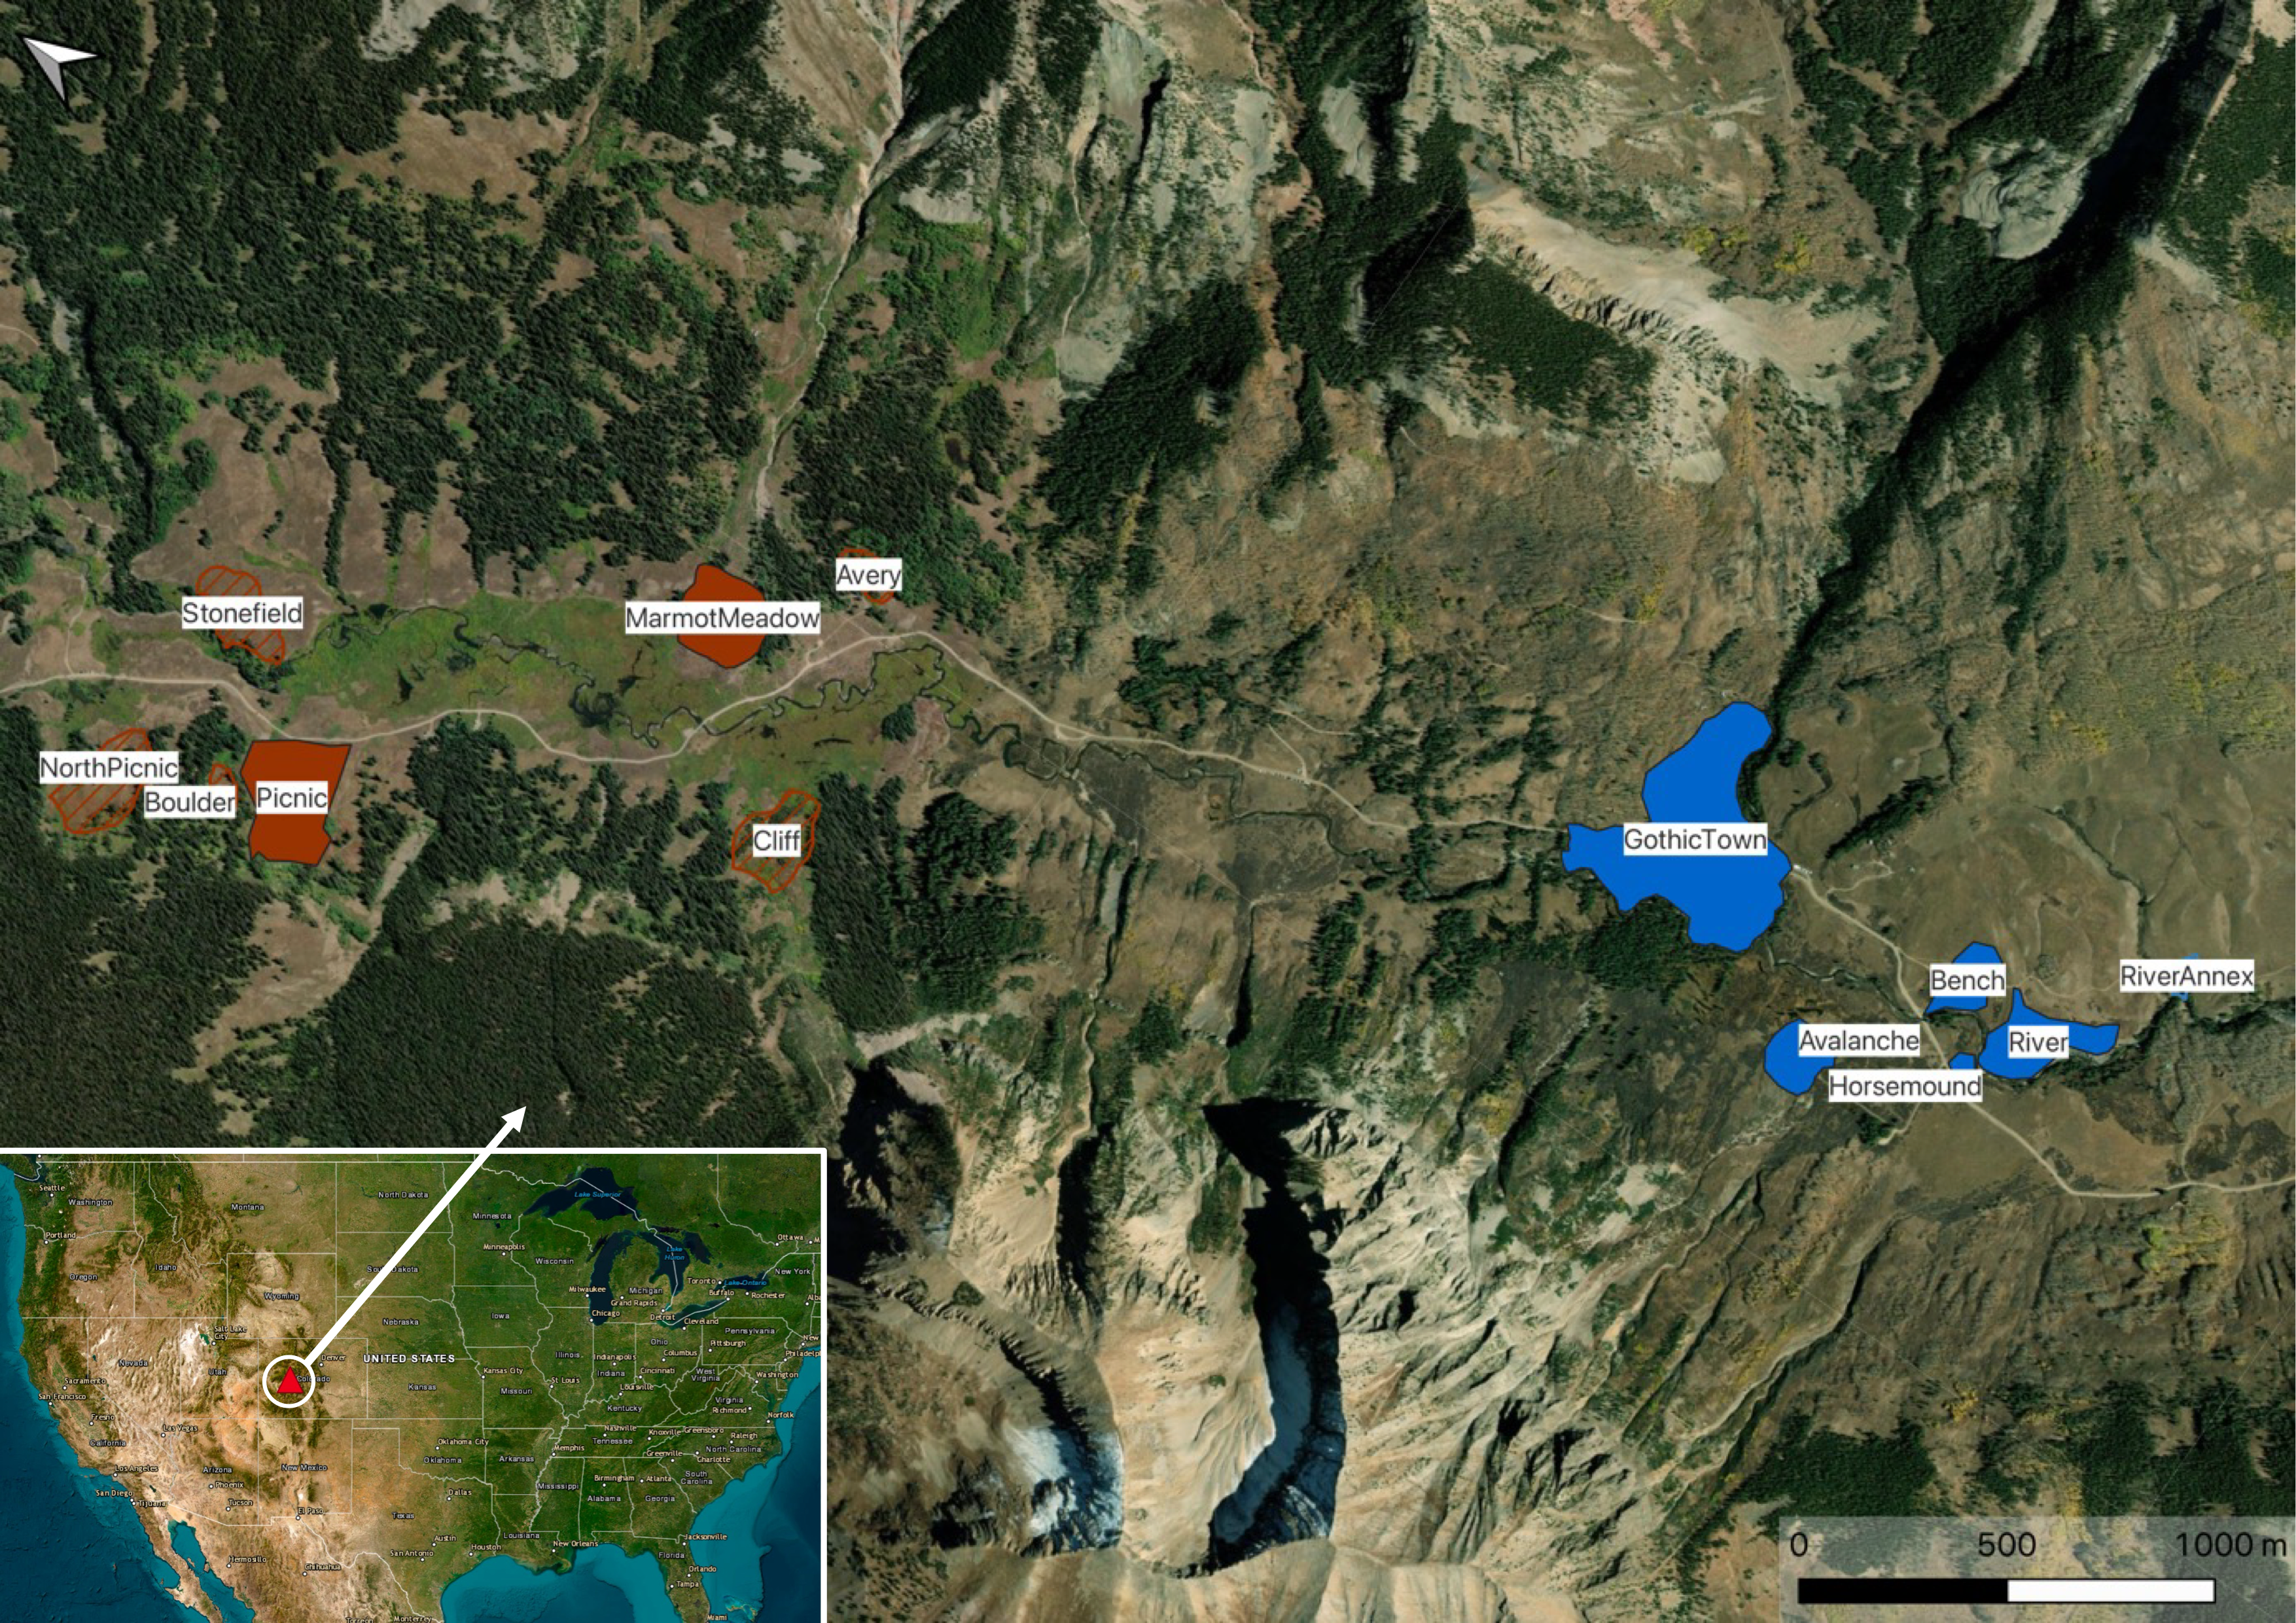
\includegraphics[keepaspectratio]{figures/map_study_site.png}}

}

\caption{\label{fig-map-study-site}Red colonies represent the ``up''
valley, blue ones represent the ``down'' valleys. Plain background
polygons represent the seven main colonies. The map was created with
QGIS software (QGIS Development Team 2024) and the base map comes from
ESRI (ESRI n.d.).}

\end{figure}%

\subsubsection{Body mass increase in yellow-bellied
marmots}\label{body-mass-increase-in-yellow-bellied-marmots}

An important body mass increase has been observed in this population
over the past half-century, estimated around \(600\ g\), representing
almost \(20\%\) of total individuals' body mass (Birot, Blumstein \&
Martin, manuscript in progress, Fig~\ref{fig-phenot}). Previous studies
concluded that most of the change was due to phenotypic plasticity
(Ozgul et al. 2010). This would a potential expectation under climate
change since the active season is getting longer and population faces
milder winter conditions (e.g., higher temperature, less snow). Hence,
marmots have more time to forage and gain weight, and the hibernation
period is getting shorter, meaning less time for individuals to lose
mass. With these new conditions, individuals are getting heavier.

However, the study by Ozgul et al. (2010) used an approach that later
proved to be flawed, not estimating genetic variance properly (Chevin
2015; Janeiro et al. 2017). With now almost 15 additional years of data,
we reanalyzed the body mass data using animal models to properly assess
the genetic change in body mass over time using body mass from 199 adult
females between 1965 and 2022 (657 observations). Our results show a
large genetic basis of body mass with a heritability of 0.56, and an
increase at the genetic level of \textasciitilde400 g over the study
period, indicating that roughly two third of the observed body mass
increase is in fact due to genetic changes (Birot et al., Manuscript in
progress, Figure~\ref{fig-genet}). With these results, it is reasonable
to conclude that plasticity is not the only process causing this
phenotypic shift, but that evolution also plays a crucial role here.

Furthermore, although the lengthening of the active season is indeed a
good potential explanation for the body mass increase through phenotypic
plasticity, it doesn't match with the observed evolutionary pattern.
Indeed, the observed increasingly milder conditions in parallel to this
change in body mass should decrease selection on body mass, as it lower
the survival pressure through hibernation. The observed body mass
increase here should be expected with an increasing pressure over winter
survival. It is clear that the lengthening active season and global
milder condition are not the only drivers of body mass changes, since we
observed both plasticity and micro-evolution.

Considering the importance of body mass for yellow-bellied marmots, it
is crucial to understand how this trait in this population is responding
to climate change, both for conservation purposes and better
understanding of the links between phenotype and environment. There is a
pressing need to explore which environmental factors may have triggered
this shift, the mechanisms behind this increase, and the potential
implications for the population's future to better understand how can
natural population cope with climate change.

\begin{figure}

\begin{minipage}{\linewidth}

\centering{

\pandocbounded{\includegraphics[keepaspectratio]{figures/fig-cohort-mod-1.png}}

}

\subcaption{\label{fig-phenot}Phenotypic change}

\end{minipage}%
\newline
\begin{minipage}{\linewidth}

\centering{

\pandocbounded{\includegraphics[keepaspectratio]{figures/fig-pbv-cohort-1.png}}

}

\subcaption{\label{fig-genet}Genetic change}

\end{minipage}%

\caption{\label{fig-A-F-bodymass}Adult females' mean cohort's body mass.
(a) At phenotypic level, trend lines (± SE) represent LMM predictions
and points shows raw data. (b) At genetic level, median trends of the
observations (red line) and under a null scenario (black line) are
represented, according to linear models, points, and error bars
represent the median and 95\% credibility interval of the posterior mean
predicted breading values for each cohort.}

\end{figure}%

\subsubsection{Data collection}\label{data-collection}

Each year between May and September since 1962, marmots are regularly
trapped (between 1 and 20 times per individual, with an average of 4.5)
using baited Tomahawk live traps (81 * 25 * 30 cm) situated near burrow
entrances. If the individual is captured for the first time, it is
identified by placing a unique pair of numbered ear tag, and with a
nontoxic black Nyzanol dye fur mark for distant identification during
behavioural observations. Over 95\% of individuals are captured during
their first 2 summers of life (as juvenile or one-year-old) and thus
have known year of birth and age. Marmot age classes can be defined as
juveniles, first year of life, yearlings as one-year-old, sub-adults as
two and three years old, and adults over 3 years old (Jebb et al. 2021).
It should be noted that sub-adults can reproduce but have not finished
their skeletal growth.

Body mass is a highly plastic trait, particularly for marmots, as it
experiences considerable fluctuations throughout the active season. It
is, for obvious reasons, impossible to record all individual body mass
at the same time. Therefore, it is necessary to estimate it for each
individual at the same time of the year. Using repeated measures for
each individual throughout each active season, a linear mixed model was
fitted and its Best Linear Unbiased Predictors were used to extract each
individual's body mass at the beginning and end of each years' active
seasons, so June 1\textsuperscript{st} and August 15\textsuperscript{th}
(Jebb et al. 2021; Martin and Pelletier 2011; details in Ozgul et al.
2010). Over 61 years of observations (1962 - 2022), we have 7,586 body
mass estimations for 4,656 individuals.

Parental links between individuals are known for most individuals in the
population (maternal links known for 3,435 individuals and paternal
links for 1,943 individuals to this date), allowing the reconstruction
of a highly detailed pedigree. Before 2002, maternal links were
estimated via behavioural observations. Since 2002, genetic parentage
assignment is used to confirm the maternal links and determine the
paternal links (details in Blumstein et al. 2010; Olson et al. 2012).

Behavioural observations and experiments (running speed and Flight
Initiation Distance (Ydenberg and Dill 1986)) are conducted all along
the season. Upon each capture, individuals are sexed, weighted
(initially with a spring scale (± 50 g) and now with a digital balance
(± 10 g)) measured and DNA samples are taken. More descriptions can be
found in Armitage (2014).

As our study site has been an important scientific station for more than
a century, we have various and exhaustive data. By combining multiple
sources of data, such as billy barr (an amateur scientist, hermit and
only year long RMBL, Phippen 2017), the National Oceanic and Atmospheric
Administration (NOAA), the United States Geological Survey (USGS), the
United States Department of Agriculture (USDA) and the Oregon State
University's PRISM Climate group, Prather et al. (2023) provides us with
exhaustive data. We have weather data (e.g., monthly temperatures,
snowing, precipitations, season lengths) at our study site from 1975 to
2022.

Data are stored in the R package ``ybamaRmot'' (Martin and Blumstein
2024), analysis will be performed in R (R Core Team 2023), Animal models
will be performed using R package asreml (Butler et al. n.d.),
lme4breeding (Covarrubias-Pazaran 2024) and MCMCglmm (Hadfield 2010),
DHGLMs and other complex models using a bayesian approach will be done
with brms (Bürkner 2021) or stan directly (Carpenter et al. 2017; Stan
Development Team et al. 2020), figures will be made with ``ggplot2''
(Wickham 2016).

\newpage{}

\subsection{Research objectives}\label{research-objectives}

The body mass increased by approximately 20\% in adults females
yellow-bellied marmots over the past 50 years. Contrary to previous
studies, I have shown during my MSc work that a large part of the change
in body mass is in fact due to micro-evolution, meaning that the
evolutionary scenario explaining this phenotypic change must be rethink
(Figure~\ref{fig-framework-objectives}).

First, I will verify how body mass has change over time across sex (male
and female), age classe (juveniles, yearling, sub-adult and adults) and
time of the year (beginning and end of the active season), at both the
phenotypic and genetic levels.

Even though our results indicate a strong genetic variation in body
mass, it doesn't explain the entire phenotypic change. Phenotypic
plasticity also plays a role here, and to fully understand the
population's reaction to climate change, we need better methods to
detect and study \emph{I * E}. Therefore, based on a simulation
approach, I am going to develop a framework to use DHGLMs to detect
\emph{I * }E* in natural conditions. I will then use this method to test
if there is individual variation in plasticity of body mass.

To continue, I will study the causes of the evolution of body mass in
this population. After having study the body mass at the beginning and
end of the active season, I will be able to test the effect of active
and hibernation seasons conditions, as well as season length on body
mass increase (during active season) and loss (during hibernation).

Finally, I will analyse the consequences of this body mass increase. I
will investigate potential behavioural changes, alongside with the
balance between body condition and experience in individual behaviour.
Understanding the link between these factor is crucial to predict
potential impacts on population dynamic in the future.

\newpage{}

\begin{figure}

\centering{

\pandocbounded{\includegraphics[keepaspectratio]{figures/framework_objectives.png}}

}

\caption{\label{fig-framework-objectives}Research objectives
illustrative framework, colour-coded by chapters research objectives.
General framework crossing over chapters is in Turquoise. Then chapter 1
is in purple, chapter 2 in yellow, Chapter 3 in green and Chapter 4 in
red.}

\end{figure}%

\newpage{}

\section{Chapter 1. Body mass increase over time, sex, age class and
time of year}\label{sec-chap1}

\begin{figure}

\centering{

\pandocbounded{\includegraphics[keepaspectratio]{figures/framework_chapter_1.png}}

}

\caption{\label{fig-framework-chapter-1}Illustration of framework for
chapter 1 focusing on evolution of body mass across sex, age and time of
the year in yellow-bellied marmots.}

\end{figure}%

For my first chapter I will study how body mass has changed in this
population over the study period across sexes, age classes and time of
year (Figure~\ref{fig-framework-chapter-1}). We know that body mass at
the end of the active season (estimated on August
15\textsuperscript{th}) has increased for adult females at both
phenotypic and genetic level (Birot, Blumstein \& Martin, manuscript in
progress). However, we still don't know how the body mass of adult
females at the beginning of the active season (estimated on June
1\textsuperscript{st}) varied over the same time period, nor for the
other age classes, nor for males. It is crucial to consider that
selective pressure, genetic structure and evolution could be different
over different sex and age classes. We need to consider the ``missing
fraction'' (i.e., bias occurring from a specific kind of viability
selection resulting in an adult population including only a certain
subset of phenotypes, Mittell and Morrissey 2024) in order to conduct a
comprehensive study of the selection acting on marmots body mass (Grafen
1988; Hadfield 2008; Jebb et al. 2021).

Juvenile body mass was predicted to stay stable as it favours a higher
running speed, allowing juveniles to escape predators more efficiently
and so spending more time foraging. On the contrary, selection was
expected for a larger body mass on adults, which rely on social
vigilance to avoid predators. This expected stabilizing selection on
juvenile body mass was the main explanation for a stable body mass in
adults marmots (Jebb et al. 2021). However, with our new results on
adult females, we now need to study potential body mass changes and
evolution for each age class.

Additionally, we have studied body mass at the end of the active season
(August 15\textsuperscript{th}), but we also have data at the emergence
from hibernation (June 1\textsuperscript{st}). We need to analyze
potential changes, at both phenotypic and genetic scale, at emergence to
better understand our population response to climate change.

A preliminary analysis looking at the body mass in juvenile cohorts over
the study period for both males and females reveals interesting details
(Figure~\ref{fig-juvenile-trend}). We see that though the mass at birth
is indeed relatively stable (or even slightly decreasing), the mass at
the end of the individuals first active season shows a similar pattern
found in adult females (i.e., cubic effect,
Figure~\ref{fig-A-F-bodymass}), although the decrease at the end of the
period seems much more pronounced here. Indeed, the body mass at the end
of our juveniles' first foraging season has increased from
\emph{1,130.64 g in 1979} to \emph{1,363.03 g in 2001}
(\emph{Estimations from local regression on raw data}). These changes
represent a body mass increase of 21\% in 22 years (22 cohorts), meaning
that between the late 1970s and early 2000s, each cohort was almost 1\%
heavier than the last one at the end of their first foraging season
(Figure~\ref{fig-juvenile-trend}).

\begin{figure}

\centering{

\pandocbounded{\includegraphics[keepaspectratio]{figures/fig-juvenile-trend-F.png}}

}

\caption{\label{fig-juvenile-trend}Body mass trend over time cohort for
female juveniles compared between the beginning (birth weight) and end
of their first active season (mass on August 15th).}

\end{figure}%

Therefore, I will analyze the changes in body mass over the study period
for all age classes at the beginning and end of the active season at
both the phenotypic and genetic level.

To do so, I will use our extensive data set in which we have body mass
estimations on June 1\textsuperscript{st} and August
15\textsuperscript{th} for 1,119 juveniles over 49 years (between 1965
and 2017); 552 yearlings over 52 years (between 1965 and 2018 \& born
between 1964 and 2017); 257 sub-adults over 49 years (between 1965 and
2019 \& born between 1963 and 2017); and for 199 adults with 657
observations over 57 years (between 1965 and 2022 \& born between 1962
and 2017), giving a total of 1,211 different individuals, with parental
links known for most of them.

At first, I will look at the variation at a phenotypic scale over time
cohorts (individuals year of birth) multivariate linear models to
account for correlations between age class.

\begin{equation}\phantomsection\label{eq-mod1-ch1}{
\begin{pmatrix}
Body\ mass\ June_{Juveniles} \\
\\
Body\ mass\ June_{Yearlings} \\
\\
Body\ mass\ June_{sub-adults} \\
\\
Body\ mass\ June_{Adults}
\end{pmatrix}
\sim
\begin{aligned}
\textbf{Fixed} &= Valley + Age \\
\\
\textbf{Random} &= Animal + UID + Measurement\ year
\end{aligned}
}\end{equation}

Then, In order to conduct a comprehensive study of the selection acting
body mass, I will use multivariate animal models to estimate genetic
covariation between each age classes for the body mass at emergence,
(Equation~\ref{eq-mod1-ch1})

\begin{equation}\phantomsection\label{eq-mod2-ch1}{
\begin{pmatrix}
Body\ mass\ August_{Juveniles} \\
\\
Body\ mass\ August_{Yearlings} \\
\\
Body\ mass\ August_{sub-adults} \\
\\
Body\ mass\ August_{Adults}
\end{pmatrix}
\sim
\begin{aligned}
\textbf{Fixed} &= Valley + Age \\
\\
\textbf{Random} &= Animal + UID + Measurement\ year
\end{aligned}
}\end{equation}

and before emergence (Equation~\ref{eq-mod2-ch1}). These models will
allow me to estimate the genetic value of the body mass over time cohort
and over the different valleys, while taking into account the
environment and within year variability. From these models, I will be
able to extract the estimated genetic variance-covariance matrices
(``G-matrix''), allowing me to check for potential antagonistic
pleiotropy (i.e., a specific case of balanced selection where fitness in
early life is maximized at the expense of fitness in later life, Hedrick
1999). I will test for that pleiotropy by looking at the body mass'
genetic covariance between the different age classes.

\newpage{}

\section{Chapter 2. Detecting individual variation in plasticity with
DHGLMs}\label{sec-chap2}

\begin{figure}

\centering{

\pandocbounded{\includegraphics[keepaspectratio]{figures/framework_chapter_2.png}}

}

\caption{\label{fig-framework-chapter-2}Illustration of framework for
chapter 2 focusing on plasticity of body mass across years in
yellow-bellied marmots.}

\end{figure}%

Detecting individual variation in plasticity is challenging due to the
unknown aspect of the environmental variables organism are responding to
(Nussey et al. 2007; Ramakers et al. 2023). Although some methods
exists, a lot of biases coming from environmental proxies still limit
these methods. DHGLMs are a promising avenue to help the study of
\emph{I * E} in natural populations, but an investigation to reveal its
potential and limits is needed.

When fitting a DHGLM on a focal phenotypic trait with multiple
observations for each individual and all individuals have experienced
the same variation in the environment, in absence of \emph{I * E} (i.e.,
each individual will exhibit the same phenotypic response,
Figure~\ref{fig-ie-vs-no-ie} a) we expect to see no among-individual
variance in the residual variance (\(V_{V_e} = 0\),
Figure~\ref{fig-ie-vs-no-ie} c).

However, if there's individual variation in plastic responses (\emph{I *
E}) for the focal phenotypic trait (Figure~\ref{fig-ie-vs-no-ie} b) and
it is not modelled with a reaction norm then the within-individual
residual variance won't be the same for each individual, hence
\(V_{V_e}\) will be different from 0 (Figure~\ref{fig-ie-vs-no-ie} d).

\begin{figure}

\centering{

\pandocbounded{\includegraphics[keepaspectratio]{figures/chapter_2.png}}

}

\caption{\label{fig-ie-vs-no-ie}Reaction norms (a,c,e) and phenotypic
variance (b,d,f) for two individuals (blue and yellow) for a trait
without (a,e) and with (c) individual variations in plasticity. In the
absence of \emph{I * E}, both individual express the same range of
phenotypic values. However, with \emph{I * E} (d), or with an unbalanced
design (f) individuals express different range of values.}

\end{figure}%

Although detecting that \(V_{V_e}\) is different from 0 isn't a proof of
\emph{I * E} in itself, as the variation could be due to other
processes, it is a necessary condition of \emph{I * E}. Finding
\(V_{V_e} > 0\) would thus suggest that investigating I * E and looking
for the unknown E is a worthwhile investigation.

Finally, it is worth noting a potential bias with this method that must
be taken into account when performing such analysis. When individuals
are sampled on different range of environmental values then the
within-indivdiual variance in residual variance could be different from
zero despite an absence of \emph{I * E} (Figure~\ref{fig-ie-vs-no-ie} e,
f). However, adding the environment as a fixed effect in the model would
remove this bias.

Based on that, I will simulate phenotypic and environmental values for
populations with and without \emph{I * E}, with balanced and unbalanced
environmental conditions. On these simulated data, I will fit DHGLMs
models, in a Bayesian framework using R package, brms (Bürkner 2021),
and stan software (Carpenter et al. 2017; Stan Development Team et al.
2020). I will also investigate the potential use of TMB (Kristensen et
al. 2016) which allows to fit DHGLMs using a frequentist approach which
is much faster especially in a simulation setup, but it relies on a
different coding language (mix of R and C).

Then, I will then apply this method on our Yellow-Bellied Marmots
population to illustrate it with a real condition example. Although my
preliminary MSc work showed that the majority of the body mass increase
rely on a genetic change and is therefore an evolution, our estimations
indicate that still a significant amount (approx. 40\%) of this change
is cause by plasticity. Ozgul et al. (2010) already proposed that his
was caused by longer active seasons giving individuals more time to
forage. But, to our knowledge, this plasticity in bodyy mass haven't
been studied at the individual level, and individual variation in
plasticity is yet to be tested. Hence, I am planning to apply DHGLM look
for potential I * E in body mass in our population of Yellow-Bellied
Marmots (Figure~\ref{fig-framework-chapter-2}).

\newpage{}

\section{Chapter 3. Identifying predictors of increased body
mass}\label{sec-chap3}

\begin{figure}

\centering{

\pandocbounded{\includegraphics[keepaspectratio]{figures/framework_chapter_3.png}}

}

\caption{\label{fig-framework-chapter3}Illustration of framework for
chapter 3 focusing on potential predictors of increased body mass in
yellow-beliied marmot.}

\end{figure}%

If we look at the climate harshness variation at our study site in the
last 50 years, as expected with climate change, we see a clear tendency
to warmer and milder years through time
(Figure~\ref{fig-climate-variation}).

\begin{figure}

\begin{minipage}{0.50\linewidth}

\centering{

\pandocbounded{\includegraphics[keepaspectratio]{figures/climate-corcircle.png}}

}

\subcaption{\label{fig-corcircle}PCA correlation circle}

\end{minipage}%
%
\begin{minipage}{0.50\linewidth}

\centering{

\pandocbounded{\includegraphics[keepaspectratio]{figures/fig-seasonal-gradient.png}}

}

\subcaption{\label{fig-sg}Temporal variation}

\end{minipage}%

\caption{\label{fig-climate-variation}Climatic variation at RMBL from
1975 to 2013. I conducted a Principal Component Analysis (PCA) using
``ade4'' package (Dray et al. 2023) over 10 weather variables. (a) We
interpret the first axis as a ``seasonal gradient'' with high values
being associated with years of long and cold winter, and low values
associated to milder years, with longer active seasons. (b) After
extracting seasonal gradient for each year from 1975 to 2013, we can
explore the temporal tendency of climatic conditions at study site
(Birot et al., manuscript in progress).}

\end{figure}%

At first sight, evolution toward a bigger body mass in marmots seems
expected. Indeed, bigger body mass is associated with better fitness as
it increases probability of survival over hibernation (Jebb et al. 2021;
Ozgul et al. 2010). The main selective event being hibernation. However,
here, we have selection for bigger body mass, in a period where the
selective pressure from hibernation is decreasing due to warmer and
milder winters (Figure~\ref{fig-paradox-chapter-3}). Hence, we face some
sort of paradox, where evolution seems to occur when the presumed
driving selective pressure is decreasing.

\begin{figure}

\centering{

\pandocbounded{\includegraphics[keepaspectratio]{figures/paradox_chapter_3.png}}

}

\caption{\label{fig-paradox-chapter-3}Evolutionary paradox behind body
mass increase.}

\end{figure}%

Changing season length is a good explanation for the body mass increase
through plasticity, individuals having more time to forage. But, this
paradox justifies further research to identify the selective pressures
driving the observed body mass evolution.

The first step is going to be to gather environmental data. I will be
able to extract and estimate hibernation and active season length,
seasonal conditions (average snowpacks, average temperatures and
precipitation), food availability, and drought frequency and severity
over the last 50 years (Figure~\ref{fig-framework-chapter3}).

Then from the body mass at the beginning and the end of the active
season, I will also be able to estimate the body mass gained in an
active season (mass in August minus mass in June), but also the mass
loss during hibernation (mass in June minus mass in August in previous
year).

\begin{equation}\phantomsection\label{eq-mod-ch3}{
\begin{pmatrix}
Body\ mass\ gain \\
\\
Body\ mass\ loss
\end{pmatrix}
\sim
\begin{aligned}
\textbf{Fixed} &= Seasonal\ conditions + Age + Drought \\
&+ Food + Season\ lengths \\
\\
\textbf{Random} &= Animal + UID + Measurement\ year
\end{aligned}
}\end{equation}

I will then begin by examine temporal trend for both environmental and
body mass data. I will also estimate the genetic variance covariance
between mass gain and mass loss using bivariate animal models. And
finally, I am going to test the effect of the different environmental
data, while controlling for individuals' age
(Equation~\ref{eq-mod-ch3}).

\newpage{}

\section{Chapter 4. Balance between body condition and experience as
predictors of marmots' behaviour}\label{sec-chap4}

\begin{figure}

\centering{

\pandocbounded{\includegraphics[keepaspectratio]{figures/framework_chapter_4.png}}

}

\caption{\label{fig-framework-chapter-4}Illustration of framework for
chapter 4 focusing on the effects of body mass increase and life
experience yellow-bellied marmots' behaviour.}

\end{figure}%

In the context of the extended pace of life syndrome framework (Dammhahn
et al. 2018; Réale et al. 2010), we expect correlation between body mass
and individuals' behaviour. Evidences has been found for a link between
body mass and individual behaviour in our marmots population from
openfield experiments (Petelle et al. 2019). As explained and emphasized
by Lande and Arnold (1983) and Teplitsky et al. (2014), understanding
the evolution of a trait requires accounting for potential correlations
with other traits. Therefore, to better understand what is happening for
both body mass and behaviour in this population, it is necessary to
study the evolution of each traits as well as their genetic and
phenotypic correlation (Figure~\ref{fig-framework-chapter-4}).

In addition to that we also expect that behaviour and personality will
be impacted by life experience and change through an individual's life
(Stamps and Groothuis 2010).

In our population, for example, the proportion of time ``stand looking''
seems to be more impacted by body mass during the two first years of
life than it is for adults (Figure~\ref{fig-prop-slook}).

\begin{figure}

\centering{

\pandocbounded{\includegraphics[keepaspectratio]{figures/prop_slook.png}}

}

\caption{\label{fig-prop-slook}Proportion of time spent stand looking
(within two-minute focal observations) as a function of scaled mass on
August 15th across age classes: Juveniles (0-1 year), Yearlings (1-2
years), sub-adults (2-3 years), and Adults (3+ years). Red lines
represent local regressions, and points represent raw data.}

\end{figure}%

Although the impact of body mass, with bigger individuals spending more
time looking is easily explainable as heavier individuals are slower and
thus must stay more vigilant to avoid predation, this age effect is
interesting to note and advocate for the hypothesis that with age,
experience could prevail on physical condition to dictate behaviour,
with older individuals more careful than juveniles, as already suggested
by Jebb et al. (2021).

\begin{equation}\phantomsection\label{eq-mod-ch4-m1}{
Boldness
\sim
\begin{aligned}
\textbf{Fixed} &= Cohort \\
\\
\textbf{Random} &= Animal + UID + Measurement\ year_{Factor}
\end{aligned}
}\end{equation}

We have repeated observations for a lot of individuals over various
variables from observations from 2-min focal observations and
flight-initiation distance experiments. I am going to reassess the
repeatability (using mixed models) of each of these variables, then look
at the correlation between those variables to determine individual
values for various personality traits such as boldness (Réale et al.
2007). Then I will determine the heritability of each of these traits
(using animal models, Equation~\ref{eq-mod-ch4-m1}).

\begin{equation}\phantomsection\label{eq-mod-ch4-m2}{
\begin{pmatrix}
Boldness \\
\\
Body\ mass
\end{pmatrix}
\sim
\begin{aligned}
\textbf{Fixed} &= Cohort \\
\\
\textbf{Random} &= Animal + UID + Measurement\ year_{Factor}
\end{aligned}
}\end{equation}

Then, I will estimate the genetic correlation between those personality
traits and body mass over cohorts using a bivariate animal model
(Equation~\ref{eq-mod-ch4-m2}).

\begin{equation}\phantomsection\label{eq-mod-ch4-m3}{
Boldness
\sim
\begin{aligned}
\textbf{Fixed} &= Body\ mass * Age + Cohort \\
\\
\textbf{Random} &= UID + Measurement\ year_{Factor}
\end{aligned}
}\end{equation}

Finally, I will test the effect of the interaction between body mass and
individual age while accounting for time cohort variation and
controlling for individual and measurement year effects, using LMM
(Equation~\ref{eq-mod-ch4-m3}).

In addition, the marmot population seems to be increasing since the
2000s (Ozgul et al. 2010). Furthermore, it is known that both body mass
(Ozgul et al. 2010), but also behaviour (Réale et al. 2007; Wolf and
Weissing 2012) can impact population dynamics. It is therefore crucial
to study the relation between body mass, behaviour, and population
dynamics to better understand, and predict, future implications of this
body mass increase for our population in a context of climate change.

\newpage{}

\section{Significance and impacts}\label{sec-signif}

This project provide a rare opportunity to study a remarkable response
to climate change at both phenotypic and genetic levels. The observed
body mass increase in Yellow-Bellied Marmots -representing a substantial
20\% rise in adult females occurred at a notable speed, seemingly, three
decades, between the 1970s and the early 2000s.

Using one of the most extensive and detailed long-term datasets on a
natural population, this research enables an unparalleled exploration of
wild populations' response to climate change. This research allows for
complex and powerful analyses, typically unfeasible in natural systems.

By investigating how the body mass has changed (i.e., basis constitution
or growing capacity), developing new methods to detect individual
variation in plasticity, and identifying predictors of this shift, this
research will contribute crucial knowledge about the complex interplay
between genotype, phenotype, and environment. Furthermore, exploring the
balance between body condition and life experience as predictors of
individual behaviour will improve our understanding of adaptive
strategies in wild population.

By studying how natural population respond to rapidly changing
environmental conditions, this project aims to give critical insights
for conservations strategies and predictions. Understanding the causes
and consequences of phenotypic response to climate change is essential
for predicting future viability of natural populations.

We hope that findings from this research will help inform conservation
policymakers by improving projections of species' adaptive capacity and
resilience to climate change, offering guidance for managing
biodiversity in a rapidly changing world.

\newpage{}

\section{Potential side projects}\label{sec-side-proj}

\begin{enumerate}
\def\labelenumi{\arabic{enumi}.}
\tightlist
\item
  Buffer environmental instability by increasing your body mass: an
  application of conservative bet-hedging in a hibernant rodent.
\end{enumerate}

When producing offspring, bet-hedging strategy correspond to ``bet'' on
the best fitness for the long term, at the expense of immediate fitness,
in order to cope with an unpredictable environment (Childs et al. 2010;
Philippi and Seger 1989; Starrfelt and Kokko 2012).

Bet-hedging strategy can be of two types, either diversified bet-hedging
(usually explained with the adage ``don't put all your eggs in the same
basket''), corresponding to increasing phenotypic variance in offspring,
increasing the chance that at least some of them will be adapted to the
condition they will face, and therefore assuring gene transmission to
next generations (Cohen 1966; Rajon et al. 2014); or conservative
bet-hedging (explained by the adage ``one bird in the hand is worth two
in the bush''), corresponding to lower fitness (i.e., number of
offsprings) variation, which can be costly in years with good conditions
as the fitness isn't maximized, but more secured in poor years, as the
fitness is less variable (Einum and Fleming 2004; Philippi and Seger
1989).

With climate change, environment are less predictable than ever. To cope
with that unpredictability, conservative bet-hedging is expected to be a
relevant adaptive strategy (Einum and Fleming 2004).

Applied to body mass, conservative bet-hedging would correspond to the
production of less but bigger offspring, and a reduced variance in the
offspring phenotype. The costs on immediate fitness for the parent is
that in a good year, more offspring could have been produced, assuring
more gene transmission. However, in poor years, the chances that
offspring will survive is greater (Philippi and Seger 1989).

For the marmots, bigger individuals would have more chance to survive
over hibernation and therefore participate in the next breeding season.
With environment becoming less and less predictable, especially at high
altitude (Inouye and Wielgolaski 2003), conservative bet-hedging can be
seen as an insurance. With that strategy, fitness will be less variable
as it is less impacted by the quality of the year in terms of resources,
bigger individuals being able to buffer poor years. This decreasing
fitness variability over time is predicted to be favoured by selection
(Cohen 1966; Einum and Fleming 2004).

I will use a simulation based approach simulating different strategies
(bet-hedging vs not bet-hedging) parametrized on the observed population
at RMBL. At first, I will compare fitness geometric mean (Philippi and
Seger 1989) over the period for the two simulated populations. This will
allow me to test if the two strategies have different outcomes and if so
which strategy would be the best in our habitat.

Although conservative bet-hedging for fewer but bigger offspring has
been predicted to be a good strategy to cope with unpredictable
environment, if it becomes too variable, simulations shows that
diversified bet-hedging becomes a better option (Einum and Fleming
2004). Indeed, the population can mismatch with its environment
(Stenseth and Mysterud 2002; Visser and Both 2005). Then, if phenotypic
variation has decreased too much, the population looses its adaption
capacity and finds itself in an ``evolutionary trap'' (Robertson et al.
2013; Schlaepfer et al. 2002).

\begin{enumerate}
\def\labelenumi{\arabic{enumi}.}
\setcounter{enumi}{1}
\tightlist
\item
  Identify key patches for meta-population persistence using Social
  Network Analysis methods. \emph{(Continuation of a project previously
  started at NTNU with Dr.~Yimen Araya-Ajoy)}
\end{enumerate}

A meta-population is defined as a set of subpopulations distributed
across various patches, more or less interconnected. Links between
subpopulations (i.e., migration fluxes) in a meta-populations is crucial
for its survival over time, as it maintains genetic diversity. If a
subpopulation finds itself isolated from the rest of the network, lack
of genetic diversity putting it at risk of extinction.

To various extent, a meta-population can be viewed as a population-scale
network (i.e., a set of patches connected by edges of varying intensity,
Krause et al. 2015). Therefore, Social Network Analysis can offer a
valuable approach to study meta-population dynamics by identifying key
patches contributing to network connectivity and resilience (Farine and
Whitehead 2015).

Using data from a long-term study on a wild house sparrow
meta-population inhabiting an archipelago in the district Helgeland,
northern Norway, I conducted preliminary analysis to test these
analyses. Initial findings (e.g., non-random structural patterns and
hierarchical order in island selection for emigration, independent of
geographic distance) provides encouraging insight about migratory
behaviour within meta-population.

Focus on understanding the migration dynamics and identifying critical
patches in meta-population can offer insight for policy makers. We hope
to develop new methods allowing to take effective measures, applicable
more efficiently with less need of extensive data. This would help to
preserve meta-population, safeguarding genetic diversity, connectivity,
and better understanding their resilience capacity in context of
changing environment.

\newpage{}

\section{Expected Products}\label{expected-products}

\textbf{Introduction} \emph{(French MSc second year project)}

\begin{enumerate}
\def\labelenumi{\arabic{enumi}.}
\tightlist
\item
  \emph{Just plasticity, are you sure?} Evidence for a strong increase
  of body mass predicted breeding values in yellow-bellied marmots over
  the last half century. \ul{A Birot, D Blumstein and JGA Martin}
  \emph{Prepared for Evolution}
\end{enumerate}

\textbf{Thesis}

\begin{enumerate}
\def\labelenumi{\arabic{enumi}.}
\setcounter{enumi}{1}
\item
  Towards more comprehensive studies of phenotypic changes: Addressing
  the missing fraction problem of changing body mass in yellow-bellied
  marmots. \ul{A Birot, D Blumstein and JGA Martin}. Targeted journal:
  \emph{Evolution}
\item
  Break free from bad environmental proxies when studying I * E, the
  DHGLMs solution. \ul{A Birot, N Dochtermann and JGA Martin}. Targeted
  journal: \emph{Methods in Ecology and Evolution}
\item
  Which part of climate change drives the evolution of body mass in
  yellow-bellied marmots? \ul{A Birot, D Blumstein and JGA Martin}.
  Targeted journal: \emph{Ecology and Evolution}
\item
  From mass to manner: How body mass and age shape behaviour in
  yellow-bellied marmots. \ul{A Birot, D Blumstein and JGA Martin}.
  Targeted journal: \emph{The American Naturalist}
\end{enumerate}

\textbf{Side projects}

\begin{enumerate}
\def\labelenumi{\arabic{enumi}.}
\setcounter{enumi}{5}
\item
  Buffer environmental instability by increasing your body mass: An
  application of conservative bet-hedging in a hibernant rodent. \ul{A
  Birot, D Blumstein and JGA Martin}. Targeted journal: \emph{Ecology
  and Evolution}
\item
  Identify key patches for meta-population persistence using Social
  Network Analysis methods. \ul{A Birot, B-E Sæther, H Jensen, J Wright,
  (JGA Martin), Y Araya-Ajoy}. Targeted journal: \emph{Methods in
  Ecology and Evolution}
\end{enumerate}

\newpage{}

\section{Timeline}\label{timeline}

\begin{figure}

\centering{

\pandocbounded{\includegraphics[keepaspectratio]{figures/gantt_24_25.png}}

\pandocbounded{\includegraphics[keepaspectratio]{figures/gantt_25_26.png}}

}

\caption{\label{fig-timeline-first}Proposed timeline for the first and
second year.}

\end{figure}%

\begin{figure}

\centering{

\pandocbounded{\includegraphics[keepaspectratio]{figures/gantt_26_27.png}}

\pandocbounded{\includegraphics[keepaspectratio]{figures/gantt_27_28.png}}

}

\caption{\label{fig-timeline-second}Proposed timeline for the third and
fourth year.}

\end{figure}%

\newpage{}

\section{References}\label{references}

\phantomsection\label{refs}
\begin{CSLReferences}{1}{0}
\bibitem[\citeproctext]{ref-acquaroneEffectsFoodAbundance2002}
Acquarone, C., Cucco, M., Cauli, S. L., and Malacarne, G. (2002),
{``Effects of food abundance and predictability on body condition and
health parameters: {Experimental} tests with the {Hooded Crow},''}
\emph{Ibis}, 144.
\url{https://doi.org/10.1046/j.1474-919X.2002.t01-2-00094_1.x}.

\bibitem[\citeproctext]{ref-alerstamBirdMigration2004}
Alerstam, T., and Christie, D. A. (2004), \emph{Bird migration},
Cambridge University Press.

\bibitem[\citeproctext]{ref-archieDominanceRankRelationships2006}
Archie, E. A., Morrison, T. A., Foley, C. A. H., Moss, C. J., and
Alberts, S. C. (2006), {``Dominance rank relationships among wild female
{African} elephants, {Loxodonta} africana,''} \emph{Animal Behaviour},
71, 117--127. \url{https://doi.org/10.1016/j.anbehav.2005.03.023}.

\bibitem[\citeproctext]{ref-armitageVernalBehaviourYellowbellied1965}
Armitage, K. B. (1965), {``Vernal behaviour of the yellow-bellied marmot
({Marmota} flaviventris),''} \emph{Animal Behaviour}, 13, 59--68.
\url{https://doi.org/10.1016/0003-3472(65)90072-2}.

\bibitem[\citeproctext]{ref-armitageMarmotBiologySociality2014}
Armitage, K. B. (2014), \emph{Marmot {Biology}: {Sociality}, {Individual
Fitness}, and {Population Dynamics}}, Cambridge University Press.
\url{https://doi.org/10.1017/CBO9781107284272}.

\bibitem[\citeproctext]{ref-arnoldAdaptiveLandscapeConceptual2001}
Arnold, S. J., Pfrender, M. E., and Jones, A. G. (2001), {``The adaptive
landscape as a conceptual bridge between micro- and macroevolution,''}
in \emph{Microevolution {Rate}, {Pattern}, {Process}}, eds. A. P. Hendry
and M. T. Kinnison, Dordrecht: Springer Netherlands, pp. 9--32.
\url{https://doi.org/10.1007/978-94-010-0585-2_2}.

\bibitem[\citeproctext]{ref-bellCostsReproductionTheir1980}
Bell, G. (1980), {``The {Costs} of {Reproduction} and {Their
Consequences},''} \emph{The American Naturalist}, 116, 45--76.
\url{https://doi.org/10.1086/283611}.

\bibitem[\citeproctext]{ref-bergmannRelationshipsHeatConservation1847}
Bergmann (1847), {``About the relationships between heat conservation
and body size of animals,''} \emph{Goett Stud}, 1, 595--708.

\bibitem[\citeproctext]{ref-bieberBodyMassDependent2014}
Bieber, C., Lebl, K., Stalder, G., Geiser, F., and Ruf, T. (2014),
{``Body mass dependent use of hibernation: {Why} not prolong the active
season, if they can?''} \emph{Functional Ecology}, (C. Franklin, ed.),
28, 167--177. \url{https://doi.org/10.1111/1365-2435.12173}.

\bibitem[\citeproctext]{ref-biroAreAnimalPersonality2008}
Biro, P. A., and Stamps, J. A. (2008), {``Are animal personality traits
linked to life-history productivity?''} \emph{Trends in Ecology \&
Evolution}, 23, 361--368.
\url{https://doi.org/10.1016/j.tree.2008.04.003}.

\bibitem[\citeproctext]{ref-blumsIndividualQualitySurvival2005}
Blums, P., Nichols, J. D., Hines, J. E., Lindberg, M. S., and Mednis, A.
(2005), {``Individual quality, survival variation and patterns of
phenotypic selection on body condition and timing of nesting in
birds,''} \emph{Oecologia}, 143, 365--376.
\url{https://doi.org/10.1007/s00442-004-1794-x}.

\bibitem[\citeproctext]{ref-blumsteinSocialEffectsEmergence2009}
Blumstein, D. T. (2009), {``Social effects on emergence from hibernation
in yellow-bellied marmots,''} \emph{Journal of Mammalogy}.

\bibitem[\citeproctext]{ref-blumsteinYellowbelliedMarmotsMarmota2004}
Blumstein, D. T., Im, S., Nicodemus, A., and Zugmeyer, C. (2004),
{``Yellow-bellied {Marmots} ({Marmota} flaviventris) {Hibernate
Socially},''} \emph{Journal of Mammalogy}, 85, 25--29.
\url{https://doi.org/10.1644/1545-1542(2004)085\%3C0025:YMMFHS\%3E2.0.CO;2}.

\bibitem[\citeproctext]{ref-blumsteinHeritabilityAntipredatoryTraits2010}
Blumstein, D. T., Lea, A. J., Olson, L. E., and Martin, J. G. A. (2010),
{``Heritability of anti-predatory traits: {Vigilance} and locomotor
performance in marmots,''} \emph{Journal of Evolutionary Biology}, 23,
879--887. \url{https://doi.org/10.1111/j.1420-9101.2010.01967.x}.

\bibitem[\citeproctext]{ref-breuerPhenotypicCorrelatesMale2012}
Breuer, T., Robbins, A. M., Boesch, C., and Robbins, M. M. (2012),
{``Phenotypic correlates of male reproductive success in western
gorillas,''} \emph{Journal of Human Evolution}, 62, 466--472.
\url{https://doi.org/10.1016/j.jhevol.2012.01.006}.

\bibitem[\citeproctext]{ref-burknerBayesianItemResponse2021}
Bürkner, P.-C. (2021), {``Bayesian {Item Response Modeling} in
{\emph{R}} with {\textbf{Brms}} and {\emph{Stan}},''} \emph{Journal of
Statistical Software}, 100. \url{https://doi.org/10.18637/jss.v100.i05}.

\bibitem[\citeproctext]{ref-butlerASRemlEstimatesVariance}
Butler, D. G., Cullis, B. R., Gilmour, A. R., Gogel, B. J., and
Thompson, R. (n.d.). {``{ASReml} estimates variance components under a
general linear,''} \emph{VSN International Ltd., Hemel Hempstead, HP2
4TP, UK}.

\bibitem[\citeproctext]{ref-cainCompetitiveFemalesAre2012}
Cain, K. E., and Ketterson, E. D. (2012), {``Competitive females are
successful females; phenotype, mechanism, and selection in a common
songbird,''} \emph{Behavioral Ecology and Sociobiology}, 66, 241--252.
\url{https://doi.org/10.1007/s00265-011-1272-5}.

\bibitem[\citeproctext]{ref-careyMammalianHibernationCellular2003}
Carey, H. V., Andrews, M. T., and Martin, S. L. (2003), {``Mammalian
{Hibernation}: {Cellular} and {Molecular Responses} to {Depressed
Metabolism} and {Low Temperature},''} \emph{Physiological Reviews}, 83,
1153--1181. \url{https://doi.org/10.1152/physrev.00008.2003}.

\bibitem[\citeproctext]{ref-carpenterStanProbabilisticProgramming2017}
Carpenter, B., Gelman, A., Hoffman, M. D., Lee, D., Goodrich, B.,
Betancourt, M., Brubaker, M., Guo, J., Li, P., and Riddell, A. (2017),
{``Stan: {A Probabilistic Programming Language},''} \emph{Journal of
Statistical Software}, 76. \url{https://doi.org/10.18637/jss.v076.i01}.

\bibitem[\citeproctext]{ref-qg_in_the_wild}
Charmantier, A., Garant, D., and Kruuk, L. E. B. (2014),
\emph{Quantitative genetics in the wild}, Oxford University Press.
\url{https://doi.org/10.1093/acprof:oso/9780199674237.001.0001}.

\bibitem[\citeproctext]{ref-chevinEvolutionAdultSize2015}
Chevin, L.-M. (2015), {``Evolution of adult size depends on genetic
variance in growth trajectories: A comment on analyses of evolutionary
dynamics using integral projection models,''} \emph{Methods in Ecology
and Evolution}, (S. Ramula, ed.), 6, 981--986.
\url{https://doi.org/10.1111/2041-210X.12389}.

\bibitem[\citeproctext]{ref-childsEvolutionaryBethedgingReal2010}
Childs, D. Z., Metcalf, C. J. E., and Rees, M. (2010), {``Evolutionary
bet-hedging in the real world: {Empirical} evidence and challenges
revealed by plants,''} \emph{Proceedings of the Royal Society B:
Biological Sciences}, 277, 3055--3064.
\url{https://doi.org/10.1098/rspb.2010.0707}.

\bibitem[\citeproctext]{ref-cohenOptimizingReproductionRandomly1966}
Cohen, D. (1966), {``Optimizing reproduction in a randomly varying
environment,''} \emph{Journal of Theoretical Biology}, 12, 119--129.
\url{https://doi.org/10.1016/0022-5193(66)90188-3}.

\bibitem[\citeproctext]{ref-covarrubias2024lme4breeding}
Covarrubias-Pazaran, G. (2024), {``Lme4breeding: Enabling genetic
evaluation in the era of genomic data,''} \emph{bioRxiv : the preprint
server for biology}, Cold Spring Harbor Laboratory, 2024--05.

\bibitem[\citeproctext]{ref-crockerImpactBodyReserves2012}
Crocker, D. E., Houser, D. S., and Webb, P. M. (2012), {``Impact of
{Body Reserves} on {Energy Expenditure}, {Water Flux}, and {Mating
Success} in {Breeding Male Northern Elephant Seals},''}
\emph{Physiological and Biochemical Zoology}, 85, 11--20.
\url{https://doi.org/10.1086/663634}.

\bibitem[\citeproctext]{ref-dammhahnPaceoflifeSyndromesFramework2018}
Dammhahn, M., Dingemanse, N. J., Niemelä, P. T., and Réale, D. (2018),
{``Pace-of-life syndromes: A framework for the adaptive integration of
behaviour, physiology and life history,''} \emph{Behavioral Ecology and
Sociobiology}, 72, 62, s00265-018-2473-y.
\url{https://doi.org/10.1007/s00265-018-2473-y}.

\bibitem[\citeproctext]{ref-darveauAllometricCascadeUnifying2002}
Darveau, C.-A., Suarez, R. K., Andrews, R. D., and Hochachka, P. W.
(2002), {``Allometric cascade as a unifying principle of body mass
effects on metabolism,''} \emph{Nature}, 417, 166--170.
\url{https://doi.org/10.1038/417166a}.

\bibitem[\citeproctext]{ref-daufresneGlobalWarmingBenefits2009}
Daufresne, M., Lengfellner, K., and Sommer, U. (2009), {``Global warming
benefits the small in aquatic ecosystems,''} \emph{Proceedings of the
National Academy of Sciences}, 106, 12788--12793.
\url{https://doi.org/10.1073/pnas.0902080106}.

\bibitem[\citeproctext]{ref-deakinEweAreWhat2022}
Deakin, S., Festa-Bianchet, M., Miller, J. M., Pelletier, F., and
Coltman, D. W. (2022), {``Ewe are what ewe wear: {Bigger} horns, better
ewes and the potential consequence of trophy hunting on female fitness
in bighorn sheep,''} \emph{Proceedings of the Royal Society B:
Biological Sciences}, 289, 20212534.
\url{https://doi.org/10.1098/rspb.2021.2534}.

\bibitem[\citeproctext]{ref-denryterSurvivalFattestHow2022}
Denryter, K., Conner, M. M., Stephenson, T. R., German, D. W., and
Monteith, K. L. (2022), {``Survival of the fattest: {How} body fat and
migration influence survival in highly seasonal environments,''}
\emph{Functional Ecology}, 36, 2569--2579.
\url{https://doi.org/10.1111/1365-2435.14151}.

\bibitem[\citeproctext]{ref-dewittCostsLimitsPhenotypic1998}
DeWitt, T. J., Sih, A., and Wilson, D. S. (1998), {``Costs and limits of
phenotypic plasticity,''} \emph{Trends in Ecology \& Evolution}, 13,
77--81. \url{https://doi.org/10.1016/S0169-5347(97)01274-3}.

\bibitem[\citeproctext]{ref-drayAde4AnalysisEcological2023}
Dray, S., Dufour, A.-B., Thioulouse, J., Jombart, T., Pavoine, S.,
Lobry, J. R., Ollier, S., Siberchicot, A., and Chessel, D. (2023),
\emph{Ade4: {Analysis} of {Ecological Data}: {Exploratory} and
{Euclidean Methods} in {Environmental Sciences}}.

\bibitem[\citeproctext]{ref-durantClimateMatchMismatch2007}
Durant, J., Hjermann, D., Ottersen, G., and Stenseth, N. (2007),
{``Climate and the match or mismatch between predator requirements and
resource availability,''} \emph{Climate Research}, 33, 271--283.
\url{https://doi.org/10.3354/cr033271}.

\bibitem[\citeproctext]{ref-einum2004environmental}
Einum, S., and Fleming, I. A. (2004), {``Environmental unpredictability
and offspring size: {Conservative} versus diversified bet-hedging,''}
\emph{Evolutionary Ecology Research}, Evolutionary Ecology, Ltd., 6,
443--455.

\bibitem[\citeproctext]{ref-esriGISMappingSoftware}
ESRI (n.d.). {``{GIS Mapping Software}, {Location Intelligence} \&
{Spatial Analytics} {\textbar} {Esri}.''}

\bibitem[\citeproctext]{ref-farineConstructingConductingInterpreting2015}
Farine, D. R., and Whitehead, H. (2015), {``Constructing, conducting and
interpreting animal social network analysis,''} \emph{Journal of Animal
Ecology}, (S. Altizer, ed.), 84, 1144--1163.
\url{https://doi.org/10.1111/1365-2656.12418}.

\bibitem[\citeproctext]{ref-festa-bianchetMassDensityDependentReproductive1998}
Festa-Bianchet, M., Gaillard, J.-M., and Jorgenson, J. T. (1998),
{``Mass- and {Density-Dependent Reproductive Success} and {Reproductive
Costs} in a {Capital Breeder},''} \emph{The American Naturalist}.

\bibitem[\citeproctext]{ref-finlayAnalysisAdaptationPlantbreeding1963}
Finlay, K., and Wilkinson, G. (1963), {``The analysis of adaptation in a
plant-breeding programme,''} \emph{Australian Journal of Agricultural
Research}, 14, 742. \url{https://doi.org/10.1071/AR9630742}.

\bibitem[\citeproctext]{ref-gardnerDecliningBodySize2011}
Gardner, J. L., Peters, A., Kearney, M. R., Joseph, L., and Heinsohn, R.
(2011), {``Declining body size: A third universal response to
warming?''} \emph{Trends in Ecology \& Evolution}, 26, 285--291.
\url{https://doi.org/10.1016/j.tree.2011.03.005}.

\bibitem[\citeproctext]{ref-geiserHibernation2013a}
Geiser, F. (2013), {``Hibernation,''} \emph{Current Biology}, 23,
R188--R193. \url{https://doi.org/10.1016/j.cub.2013.01.062}.

\bibitem[\citeproctext]{ref-gienappEvolutionaryDynamicsResponse2014}
Gienapp, P., and Brommer, J. E. (2014), {``Evolutionary dynamics in
response to climate change,''} in \emph{Quantitative {Genetics} in the
{Wild}}, eds. A. Charmantier, D. Garant, and L. E. B. Kruuk, Oxford
University PressOxford, pp. 254--274.
\url{https://doi.org/10.1093/acprof:oso/9780199674237.003.0015}.

\bibitem[\citeproctext]{ref-giorgiElevationDependencySurface1997}
Giorgi, F., Hurrell, J. W., Marinucci, M. R., and Beniston, M. (1997),
{``Elevation {Dependency} of the {Surface Climate Change Signal}: {A
Model Study},''} \emph{Journal of Climate}, 10, 288--296.
\url{https://doi.org/10.1175/1520-0442(1997)010\%3C0288:EDOTSC\%3E2.0.CO;2}.

\bibitem[\citeproctext]{ref-gouldSpandrelsSanMarco1979}
Gould, S. J., and Lewontin, R. C. (1979), {``The spandrels of {San
Marco} and the {Panglossian} paradigm: A critique of the adaptationist
programme,''} \emph{Proceedings of the Royal Society of London. Series
B. Biological Sciences}, 205, 581--598.
\url{https://doi.org/10.1098/rspb.1979.0086}.

\bibitem[\citeproctext]{ref-grabherrClimateChangeImpacts2010}
Grabherr, G., Gottfried, M., and Pauli, H. (2010), {``Climate {Change
Impacts} in {Alpine Environments},''} \emph{Geography Compass}, 4,
1133--1153. \url{https://doi.org/10.1111/j.1749-8198.2010.00356.x}.

\bibitem[\citeproctext]{ref-grafen1988uses}
Grafen, A. (1988), {``On the uses of data on lifetime reproductive
success,''} \emph{Reproductive success. Studies of individual variation
in contrasting breeding systems}, University of Chicago Press, 454--471.

\bibitem[\citeproctext]{ref-guillemainWinteringFrenchMallard2010}
Guillemain, M., Elmberg, J., Gauthier-Clerc, M., Massez, G., Hearn, R.,
Champagnon, J., and Simon, G. (2010), {``Wintering {French Mallard} and
{Teal Are Heavier} and in {Better Body Condition} than 30 {Years Ago}:
{Effects} of a {Changing Environment}?''} \emph{AMBIO}, 39, 170--180.
\url{https://doi.org/10.1007/s13280-010-0020-9}.

\bibitem[\citeproctext]{ref-hadfieldEstimatingEvolutionaryParameters2008a}
Hadfield, J. D. (2008), {``Estimating evolutionary parameters when
viability selection is operating,''} \emph{Proceedings of the Royal
Society B: Biological Sciences}, 275, 723--734.
\url{https://doi.org/10.1098/rspb.2007.1013}.

\bibitem[\citeproctext]{ref-hadfieldMCMCMethodsMultiResponse2010}
Hadfield, J. D. (2010), {``{MCMC Methods} for {Multi-Response
Generalized Linear Mixed Models}: {The} {\textbf{MCMCglmm}} {\emph{R}}
{Package},''} \emph{Journal of Statistical Software}, 33.
\url{https://doi.org/10.18637/jss.v033.i02}.

\bibitem[\citeproctext]{ref-haramisRelationshipBodyMass1986}
Haramis, G. M., Nichols, J. D., Pollock, K. H., and Hines, J. E. (1986),
{``The {Relationship Between Body Mass} and {Survival} of {Wintering
Canvasbacks},''} \emph{The Auk}, 103, 506--514.
\url{https://doi.org/10.1093/auk/103.3.506}.

\bibitem[\citeproctext]{ref-hedrickAntagonisticPleiotropyGenetic1999}
Hedrick, P. W. (1999), {``Antagonistic pleiotropy and genetic
polymorphism: A perspective,''} \emph{Heredity}, 82, 126--133.
\url{https://doi.org/10.1038/sj.hdy.6884400}.

\bibitem[\citeproctext]{ref-heldstabHowMammalsBuffer2017}
Heldstab, S. A. (2017), {``How do mammals buffer environmental
seasonality? {The} role of brain size, body fat and allomaternal care in
dealing with energy shortage,''} PhD thesis, University of Zurich.
\url{https://doi.org/10.5167/UZH-144968}.

\bibitem[\citeproctext]{ref-hillWhatAnimalBreeding2010}
Hill, W. G., and Kirkpatrick, M. (2010), {``What {Animal Breeding Has
Taught Us} about {Evolution},''} \emph{Annual Review of Ecology,
Evolution, and Systematics}, 41, 1--19.
\url{https://doi.org/10.1146/annurev-ecolsys-102209-144728}.

\bibitem[\citeproctext]{ref-inouyeHighAltitudeClimates2003}
Inouye, D. W., and Wielgolaski, F. E. (2003), {``High {Altitude
Climates},''} in \emph{Phenology: {An} integrative {Environmental
Science}}, pp. 195--214.

\bibitem[\citeproctext]{ref-intergovernmentalpanelonclimatechangeipccClimateChange20222022}
Intergovernmental Panel On Climate Change (Ipcc) (2022), \emph{Climate
{Change} 2022 -- {Impacts}, {Adaptation} and {Vulnerability}: {Working
Group II Contribution} to the {Sixth Assessment Report} of the
{Intergovernmental Panel} on {Climate Change}}, Cambridge University
Press. \url{https://doi.org/10.1017/9781009325844}.

\bibitem[\citeproctext]{ref-janeiroRobustEvolutionaryInference2017}
Janeiro, M. J., Coltman, D. W., Festa-Bianchet, M., Pelletier, F., and
Morrissey, M. B. (2017), {``Towards robust evolutionary inference with
integral projection models,''} \emph{Journal of Evolutionary Biology},
30, 270--288. \url{https://doi.org/10.1111/jeb.13000}.

\bibitem[\citeproctext]{ref-jebbBiggerNotAlways2021}
Jebb, A. H. M., Blumstein, D. T., Bize, P., and Martin, J. G. A. (2021),
{``Bigger is not always better: {Viability} selection on body mass
varies across life stages in a hibernating mammal,''} \emph{Ecology and
Evolution}, 11, 3435--3445. \url{https://doi.org/10.1002/ece3.7304}.

\bibitem[\citeproctext]{ref-castor_jenkins}
Jenkins, S. H., and Busher, P. E. (1979), {``Castor canadensis,''}
\emph{Mammalian Species}, 1--8. \url{https://doi.org/10.2307/3503787}.

\bibitem[\citeproctext]{ref-jonassonHibernationEnergeticsFreeranging2012}
Jonasson, K. A., and Willis, C. K. R. (2012), {``Hibernation energetics
of free-ranging little brown bats,''} \emph{Journal of Experimental
Biology}, The Company of Biologists, 215, 2141--2149.
\url{https://doi.org/10.1242/jeb.066514}.

\bibitem[\citeproctext]{ref-jonesOrganismsEcosystemEngineers1994}
Jones, C. G., Lawton, J. H., and Shachak, M. (1994), {``Organisms as
{Ecosystem Engineers},''} \emph{Oikos (Copenhagen, Denmark)}, 69, 373.
\url{https://doi.org/10.2307/3545850}.

\bibitem[\citeproctext]{ref-inbook}
Kittel, T., Thornton, P. E., andrew Royle, J., and Chase, T. (2002),
{``Climates of the rocky mountains: {Historical} and future patterns,''}
in \emph{Rocky {Mountain Futures}: {An Ecological Perspective}.}, pp.
59--92. \url{https://doi.org/10.13140/RG.2.1.1683.0487}.

\bibitem[\citeproctext]{ref-krauseAnimalSocialNetworks2015}
Krause, J., James, R., Franks, D. W., and Croft, D. P. (eds.) (2015),
\emph{Animal social networks}, Oxford ; New York, NY: Oxford University
Press.

\bibitem[\citeproctext]{ref-kristensenTMBAutomaticDifferentiation2016}
Kristensen, K., Nielsen, A., Berg, C. W., Skaug, H., and Bell, B. M.
(2016), {``{\textbf{TMB}} : {Automatic Differentiation} and {Laplace
Approximation},''} \emph{Journal of Statistical Software}, 70.
\url{https://doi.org/10.18637/jss.v070.i05}.

\bibitem[\citeproctext]{ref-kruukEstimatingGeneticParameters2004}
Kruuk, L. E. B. (2004), {``Estimating genetic parameters in natural
populations using the {`animal model'},''} \emph{Philosophical
Transactions of the Royal Society of London. Series B: Biological
Sciences}, 359, 873--890. \url{https://doi.org/10.1098/rstb.2003.1437}.

\bibitem[\citeproctext]{ref-kruukStudyQuantitativeGenetics2014}
Kruuk, L. E. B., Charmantier, A., and Garant, D. (2014), {``The study of
quantitative genetics in wild populations,''} in \emph{Quantitative
{Genetics} in the {Wild}}, Oxford University PressOxford, pp. 1--15.
\url{https://doi.org/10.1093/acprof:oso/9780199674237.003.0012}.

\bibitem[\citeproctext]{ref-kruukHowSeparateGenetic2007}
Kruuk, L. E. B., and Hadfield, J. D. (2007), {``How to separate genetic
and environmental causes of similarity between relatives,''}
\emph{Journal of Evolutionary Biology}, 20, 1890--1903.
\url{https://doi.org/10.1111/j.1420-9101.2007.01377.x}.

\bibitem[\citeproctext]{ref-kurzPhysiologyThermoregulation2008}
Kurz, A. (2008), {``Physiology of {Thermoregulation},''} \emph{Best
Practice \& Research Clinical Anaesthesiology}, 22, 627--644.
\url{https://doi.org/10.1016/j.bpa.2008.06.004}.

\bibitem[\citeproctext]{ref-landeMeasurementSelectionCorrelated1983}
Lande, R., and Arnold, S. J. (1983), {``The {Measurement} of {Selection}
on {Correlated Characters},''} \emph{Evolution; international journal of
organic evolution}, {[}Society for the Study of Evolution, Wiley{]}, 37,
1210--1226. \url{https://doi.org/10.2307/2408842}.

\bibitem[\citeproctext]{ref-leeDoubleHierarchicalGeneralized2006}
Lee, Y., and Nelder, J. A. (2006), {``Double hierarchical generalized
linear models,''} \emph{Journal of the Royal Statistical Society Series
C: Applied Statistics}.

\bibitem[\citeproctext]{ref-lewontinUnitsSelection1970}
Lewontin, R. C. (1970), {``The {Units} of {Selection},''} \emph{Annual
Review of Ecology and Systematics}, Annual Reviews, 1, 1--18.

\bibitem[\citeproctext]{ref-lynchGeneticsAnalysisQuantitative1998}
Lynch, M., and Walsh, B. (1998), \emph{Genetics and {Analysis} of
{Quantitative Traits}}, Sinauer.

\bibitem[\citeproctext]{ref-mardenAssessmentEnergyReserves1994}
Marden, J. H., and Rollins, R. A. (1994), {``Assessment of energy
reserves by damselflies engaged in aerial contests for mating
territories,''} \emph{Animal Behaviour}, 48, 1023--1030.
\url{https://doi.org/10.1006/anbe.1994.1335}.

\bibitem[\citeproctext]{ref-martinMeasuringGrowthPatterns2011}
Martin, J. G. A., and Pelletier, F. (2011), {``Measuring growth patterns
in the field: {Effects} of sampling regime and methods on standardized
estimates,''} \emph{Canadian Journal of Zoology}, 89, 529--537.
\url{https://doi.org/10.1139/z11-018}.

\bibitem[\citeproctext]{ref-martinYbamaRmotDatabaseMarmot2024}
Martin, J., and Blumstein, D. (2024), \emph{{ybamaRmot}: {Database} of
the {Marmot Study} in the {East River Valley}, {Colorado}}.

\bibitem[\citeproctext]{ref-meierPopulationspecificAdjustmentAnnual2020}
Meier, C. M., Karaardıç, H., Aymí, R., Peev, S. G., Witvliet, W., and
Liechti, F. (2020), {``Population-specific adjustment of the annual
cycle in a super-swift trans-{Saharan} migrant,''} \emph{Journal of
Avian Biology}, 51, jav.02515. \url{https://doi.org/10.1111/jav.02515}.

\bibitem[\citeproctext]{ref-milnerReproductiveSuccessFailure2013}
Milner, J. M., Van Beest, F. M., Solberg, E. J., and Storaas, T. (2013),
{``Reproductive success and failure: {The} role of winter body mass in
reproductive allocation in {Norwegian} moose,''} \emph{Oecologia}, 172,
995--1005. \url{https://doi.org/10.1007/s00442-012-2547-x}.

\bibitem[\citeproctext]{ref-mittell2024missing}
Mittell, E. A., and Morrissey, M. B. (2024), {``The missing fraction
problem as an episodes of selection problem,''} \emph{Evolution;
international journal of organic evolution}, Oxford University Press US,
78, 601--611.

\bibitem[\citeproctext]{ref-monclusYellowbelliedMarmotsNot2014}
Monclús, R., Pang, B., and Blumstein, D. T. (2014), {``Yellow-bellied
marmots do not compensate for a late start: {The} role of maternal
allocation in shaping life-history trajectories,''} \emph{Evolutionary
Ecology}, 28, 721--733. \url{https://doi.org/10.1007/s10682-014-9705-z}.

\bibitem[\citeproctext]{ref-nedergaardMammalianHibernation1990}
Nedergaard, J., and Cannon, B. (1990), {``Mammalian hibernation,''}
\emph{Philosophical Transactions of the Royal Society of London. B,
Biological Sciences}, 326, 669--686.
\url{https://doi.org/10.1098/rstb.1990.0038}.

\bibitem[\citeproctext]{ref-nusseyEvolutionaryEcologyIndividual2007}
Nussey, D. H., Wilson, A. J., and Brommer, J. E. (2007), {``The
evolutionary ecology of individual phenotypic plasticity in wild
populations,''} \emph{Journal of Evolutionary Biology}, 20, 831--844.
\url{https://doi.org/10.1111/j.1420-9101.2007.01300.x}.

\bibitem[\citeproctext]{ref-ohmuraEnhancedTemperatureVariability2012}
Ohmura, A. (2012), {``Enhanced temperature variability in high-altitude
climate change,''} \emph{Theoretical and Applied Climatology}, 110,
499--508. \url{https://doi.org/10.1007/s00704-012-0687-x}.

\bibitem[\citeproctext]{ref-olsonNoEvidenceInbreeding2012}
Olson, L. E., Blumstein, D. T., Pollinger, J. R., and Wayne, R. K.
(2012), {``No evidence of inbreeding avoidance despite demonstrated
survival costs in a polygynous rodent,''} \emph{Molecular Ecology}, 21,
562--571. \url{https://doi.org/10.1111/j.1365-294X.2011.05389.x}.

\bibitem[\citeproctext]{ref-ozgulCoupledDynamicsBody2010}
Ozgul, A., Childs, D. Z., Oli, M. K., Armitage, K. B., Blumstein, D. T.,
Olson, L. E., Tuljapurkar, S., and Coulson, T. (2010), {``Coupled
dynamics of body mass and population growth in response to environmental
change,''} \emph{Nature}, 466, 482--485.
\url{https://doi.org/10.1038/nature09210}.

\bibitem[\citeproctext]{ref-petelleMixedSupportState2019}
Petelle, M. B., Martin, J. G. A., and Blumstein, D. T. (2019), {``Mixed
support for state maintaining risky personality traits in yellow-bellied
marmots,''} \emph{Animal Behaviour}, 150, 177--188.
\url{https://doi.org/10.1016/j.anbehav.2019.02.008}.

\bibitem[\citeproctext]{ref-philippi1989hedging}
Philippi, T., and Seger, J. (1989), {``Hedging one's evolutionary bets,
revisited,''} \emph{Trends in ecology \& evolution}, Elsevier Current
Trends, 4, 41--44.

\bibitem[\citeproctext]{ref-phillipsVISUALIZINGMULTIVARIATESELECTION1989}
Phillips, P. C., and Arnold, S. J. (1989), {``{VISUALIZING MULTIVARIATE
SELECTION},''} \emph{Evolution; international journal of organic
evolution}, 43, 1209--1222.
\url{https://doi.org/10.1111/j.1558-5646.1989.tb02569.x}.

\bibitem[\citeproctext]{ref-phippenHermitWhoInadvertently2017}
Phippen, J. W. (2017), {``The {Hermit Who Inadvertently Shaped
Climate-Change Science},''} \emph{The Atlantic}.

\bibitem[\citeproctext]{ref-pigliucciPhenotypicPlasticityNature2001}
Pigliucci, M. (2001), \emph{Phenotypic plasticity: {Beyond} nature and
nurture}, JHU Press.

\bibitem[\citeproctext]{ref-pigliucciEvolutionPhenotypicPlasticity2005}
Pigliucci, M. (2005), {``Evolution of phenotypic plasticity: {Where} are
we going now?''} \emph{Trends in Ecology \& Evolution}, 20, 481--486.
\url{https://doi.org/10.1016/j.tree.2005.06.001}.

\bibitem[\citeproctext]{ref-pratherClimateDataRocky2023}
Prather, R. M., Underwood, N., Dalton, R. M., Barr, B., and Inouye, B.
D. (2023), {``Climate data from the {Rocky Mountain Biological
Laboratory} (1975--2022),''} \emph{Ecology}, 104, e4153.
\url{https://doi.org/10.1002/ecy.4153}.

\bibitem[\citeproctext]{ref-qgisdevelopmentteamQGISGeographicInformation2024}
QGIS Development Team (2024), {``{QGIS Geographic Information
System},''} QGIS Association.

\bibitem[\citeproctext]{ref-base}
R Core Team (2023), \emph{R: A language and environment for statistical
computing}, Manual, Vienna, Austria: R Foundation for Statistical
Computing.

\bibitem[\citeproctext]{ref-rajonEvolutionBetHedging2014}
Rajon, E., Desouhant, E., Chevalier, M., Débias, F., and Menu, F.
(2014), {``The {Evolution} of {Bet Hedging} in {Response} to {Local
Ecological Conditions},''} \emph{The American Naturalist}, 184, E1--E15.
\url{https://doi.org/10.1086/676506}.

\bibitem[\citeproctext]{ref-ramakersProbingVariationReaction2023}
Ramakers, J. J. C., Reed, T. E., Harris, M. P., and Gienapp, P. (2023),
{``Probing variation in reaction norms in wild populations: {The}
importance of reliable environmental proxies,''} \emph{Oikos
(Copenhagen, Denmark)}, 2023, e09592.
\url{https://doi.org/10.1111/oik.09592}.

\bibitem[\citeproctext]{ref-realePersonalityEmergencePaceoflife2010}
Réale, D., Garant, D., Humphries, M. M., Bergeron, P., Careau, V., and
Montiglio, P.-O. (2010), {``Personality and the emergence of the
pace-of-life syndrome concept at the population level,''}
\emph{Philosophical Transactions of the Royal Society B: Biological
Sciences}, Royal Society, 365, 4051--4063.
\url{https://doi.org/10.1098/rstb.2010.0208}.

\bibitem[\citeproctext]{ref-realeIntegratingAnimalTemperament2007a}
Réale, D., Reader, S. M., Sol, D., McDougall, P. T., and Dingemanse, N.
J. (2007), {``Integrating animal temperament within ecology and
evolution,''} \emph{Biological Reviews}, 82, 291--318.
\url{https://doi.org/10.1111/j.1469-185X.2007.00010.x}.

\bibitem[\citeproctext]{ref-riesenfeldRoleBodyMass1981}
Riesenfeld, A. (1981), {``The role of body mass in thermoregulation,''}
\emph{American Journal of Physical Anthropology}, 55, 95--99.
\url{https://doi.org/10.1002/ajpa.1330550113}.

\bibitem[\citeproctext]{ref-robertsonEcologicalNoveltyEmergence2013}
Robertson, B. A., Rehage, J. S., and Sih, A. (2013), {``Ecological
novelty and the emergence of evolutionary traps,''} \emph{Trends in
Ecology \& Evolution}, 28, 552--560.
\url{https://doi.org/10.1016/j.tree.2013.04.004}.

\bibitem[\citeproctext]{ref-Roff1992TheEO}
Roff, D. A. (1992), {``The evolution of life histories : {Theory} and
analysis.''}

\bibitem[\citeproctext]{ref-rutbergDominanceAggressionFrequencies1990}
Rutberg, A. T., and Greenberg, S. A. (1990), {``Dominance, aggression
frequencies and modes of aggressive competition in feral pony mares,''}
\emph{Animal Behaviour}, 40, 322--331.
\url{https://doi.org/10.1016/S0003-3472(05)80927-3}.

\bibitem[\citeproctext]{ref-schlaepferEcologicalEvolutionaryTraps2002}
Schlaepfer, M. A., Runge, M. C., and Sherman, P. W. (2002),
{``Ecological and evolutionary traps,''} \emph{Trends in Ecology \&
Evolution}, 17, 474--480.
\url{https://doi.org/10.1016/S0169-5347(02)02580-6}.

\bibitem[\citeproctext]{ref-sheridanShrinkingBodySize2011}
Sheridan, J. A., and Bickford, D. (2011), {``Shrinking body size as an
ecological response to climate change,''} \emph{Nature Climate Change},
1, 401--406. \url{https://doi.org/10.1038/nclimate1259}.

\bibitem[\citeproctext]{ref-siepielskiNoEvidenceThat2019}
Siepielski, A. M., Morrissey, M. B., Carlson, S. M., Francis, C. D.,
Kingsolver, J. G., Whitney, K. D., and Kruuk, L. E. B. (2019), {``No
evidence that warmer temperatures are associated with selection for
smaller body sizes,''} \emph{Proceedings of the Royal Society B:
Biological Sciences}, 286, 20191332.
\url{https://doi.org/10.1098/rspb.2019.1332}.

\bibitem[\citeproctext]{ref-smithBehavioralTypesPredictors2010}
Smith, B. R., and Blumstein, D. T. (2010), {``Behavioral types as
predictors of survival in {Trinidadian} guppies ({Poecilia}
reticulata),''} \emph{Behavioral Ecology}, 21, 919--926.
\url{https://doi.org/10.1093/beheco/arq084}.

\bibitem[\citeproctext]{ref-smithOverwinterActivityBody1991}
Smith, D. W., Peterson, R. O., Drummer, T. D., and Sheputis, D. S.
(1991), {``Over-winter activity and body temperature patterns in
northern beavers,''} \emph{Canadian Journal of Zoology}, 69, 2178--2182.
\url{https://doi.org/10.1139/z91-304}.

\bibitem[\citeproctext]{ref-stampsGrowthmortalityTradeoffsPersonality2007}
Stamps, J. A. (2007), {``Growth-mortality tradeoffs and {`personality
traits'} in animals,''} \emph{Ecology Letters}, 10, 355--363.
\url{https://doi.org/10.1111/j.1461-0248.2007.01034.x}.

\bibitem[\citeproctext]{ref-stampsDevelopmentAnimalPersonality2010}
Stamps, J., and Groothuis, T. G. G. (2010), {``The development of animal
personality: {Relevance}, concepts and perspectives,''} \emph{Biological
Reviews}, 85, 301--325.
\url{https://doi.org/10.1111/j.1469-185X.2009.00103.x}.

\bibitem[\citeproctext]{ref-stan2020rstan}
Stan Development Team, C., and others (2020), {``{RStan}: The {R}
interface to stan,''} \emph{R package version 2.21. 2}.

\bibitem[\citeproctext]{ref-starrfeltBethedgingaTripleTradeoff2012}
Starrfelt, J., and Kokko, H. (2012), {``Bet-hedging---a triple trade-off
between means, variances and correlations,''} \emph{Biological Reviews},
87, 742--755. \url{https://doi.org/10.1111/j.1469-185X.2012.00225.x}.

\bibitem[\citeproctext]{ref-stearns92}
Stearns, S. C. (1992), \emph{The evolution of life histories}, Oxford
University Press.
\url{https://doi.org/10.1093/oso/9780198577416.001.0001}.

\bibitem[\citeproctext]{ref-stensethClimateChangingPhenology2002}
Stenseth, N. Chr., and Mysterud, A. (2002), {``Climate, changing
phenology, and other life history traits: {Nonlinearity} and
match--mismatch to the environment,''} \emph{Proceedings of the National
Academy of Sciences}, 99, 13379--13381.
\url{https://doi.org/10.1073/pnas.212519399}.

\bibitem[\citeproctext]{ref-stephensonLinkingPopulationPerformance2020}
Stephenson, T. R., German, D. W., Cassirer, E. F., Walsh, D. P., Blum,
M. E., Cox, M., Stewart, K. M., and Monteith, K. L. (2020), {``Linking
population performance to nutritional condition in an alpine
ungulate,''} \emph{Journal of Mammalogy}, (P. Barboza, ed.), 101,
1244--1256. \url{https://doi.org/10.1093/jmammal/gyaa091}.

\bibitem[\citeproctext]{ref-stockleyFemaleCompetitionIts2011}
Stockley, P., and Bro-Jørgensen, J. (2011), {``Female competition and
its evolutionary consequences in mammals,''} \emph{Biological Reviews},
86, 341--366. \url{https://doi.org/10.1111/j.1469-185X.2010.00149.x}.

\bibitem[\citeproctext]{ref-teplitskyEvolutionaryPotentialConstraints2014}
Teplitsky, C., Robinson, M. R., and Merilä, J. (2014), {``Evolutionary
potential and constraints in wild populations,''} in \emph{Quantitative
{Genetics} in the {Wild}}, eds. A. Charmantier, D. Garant, and L. E. B.
Kruuk, Oxford University PressOxford, pp. 190--208.
\url{https://doi.org/10.1093/acprof:oso/9780199674237.003.0012}.

\bibitem[\citeproctext]{ref-viaAdaptivePhenotypicPlasticity1995}
Via, S., Gomulkiewicz, R., De Jong, G., Scheiner, S. M., Schlichting, C.
D., and Van Tienderen, P. H. (1995), {``Adaptive phenotypic plasticity:
{Consensus} and controversy,''} \emph{Trends in Ecology \& Evolution},
10, 212--217. \url{https://doi.org/10.1016/S0169-5347(00)89061-8}.

\bibitem[\citeproctext]{ref-visserShiftsPhenologyDue2005}
Visser, M. E., and Both, C. (2005), {``Shifts in phenology due to global
climate change: {The} need for a yardstick,''} \emph{Proceedings of the
Royal Society B: Biological Sciences}, 272, 2561--2569.
\url{https://doi.org/10.1098/rspb.2005.3356}.

\bibitem[\citeproctext]{ref-walshAbundantGeneticVariation2009}
Walsh, B., and Blows, M. W. (2009), {``Abundant {Genetic Variation} +
{Strong Selection} = {Multivariate Genetic Constraints}: {A Geometric
View} of {Adaptation},''} \emph{Annual Review of Ecology, Evolution, and
Systematics}, 40, 41--59.
\url{https://doi.org/10.1146/annurev.ecolsys.110308.120232}.

\bibitem[\citeproctext]{ref-walshPrecipitationTemperatureTrends2022}
Walsh, C. R., and Patterson, R. T. (2022), {``Precipitation and
{Temperature Trends} and {Cycles Derived} from {Historical} 1890--2019
{Weather Data} for the {City} of {Ottawa}, {Ontario}, {Canada},''}
\emph{Environments}, 9, 35.
\url{https://doi.org/10.3390/environments9030035}.

\bibitem[\citeproctext]{ref-wangChangingLengthsFour2021}
Wang, J., Guan, Y., Wu, L., Guan, X., Cai, W., Huang, J., Dong, W., and
Zhang, B. (2021), {``Changing {Lengths} of the {Four Seasons} by {Global
Warming},''} \emph{Geophysical Research Letters}, 48, e2020GL091753.
\url{https://doi.org/10.1029/2020GL091753}.

\bibitem[\citeproctext]{ref-weibelAllometricScalingMaximal2004}
Weibel, E. R., Bacigalupe, L. D., Schmitt, B., and Hoppeler, H. (2004),
{``Allometric scaling of maximal metabolic rate in mammals: {Muscle}
aerobic capacity as determinant factor,''} \emph{Respiratory Physiology
\& Neurobiology}, 140, 115--132.
\url{https://doi.org/10.1016/j.resp.2004.01.006}.

\bibitem[\citeproctext]{ref-wickhamGgplot2ElegantGraphics2016}
Wickham, H. (2016), \emph{Ggplot2: {Elegant Graphics} for {Data
Analysis}}, Springer-Verlag New York.

\bibitem[\citeproctext]{ref-williamsUnderstandingEvolutionaryImpacts2017}
Williams, C. M., Ragland, G. J., Betini, G., Buckley, L. B., Cheviron,
Z. A., Donohue, K., Hereford, J., Humphries, M. M., Lisovski, S.,
Marshall, K. E., Schmidt, P. S., Sheldon, K. S., Varpe, Ø., and Visser,
M. E. (2017), {``Understanding {Evolutionary Impacts} of {Seasonality}:
{An Introduction} to the {Symposium},''} \emph{Integrative and
Comparative Biology}, 57, 921--933.
\url{https://doi.org/10.1093/icb/icx122}.

\bibitem[\citeproctext]{ref-wilsonEcologistsGuideAnimal2010}
Wilson, A. J., Réale, D., Clements, M. N., Morrissey, M., Postma, E.,
Walling, C., Kruuk, L., and Nussey, D. (2010), {``An ecologist's guide
to the animal model.''} \emph{The Journal of animal ecology}, 79 1,
13--26. \url{https://doi.org/10.1111/j.1365-2656.2009.01639.x}.

\bibitem[\citeproctext]{ref-wolfLifehistoryTradeoffsFavour2007}
Wolf, M., Van Doorn, G. S., Leimar, O., and Weissing, F. J. (2007),
{``Life-history trade-offs favour the evolution of animal
personalities,''} \emph{Nature}, 447, 581--584.
\url{https://doi.org/10.1038/nature05835}.

\bibitem[\citeproctext]{ref-wolfAnimalPersonalitiesConsequences2012}
Wolf, M., and Weissing, F. J. (2012), {``Animal personalities:
{Consequences} for ecology and evolution,''} \emph{Trends in Ecology \&
Evolution}, 27, 452--461.
\url{https://doi.org/10.1016/j.tree.2012.05.001}.

\bibitem[\citeproctext]{ref-ydenbergEconomicsFleeingPredators1986}
Ydenberg, R. C., and Dill, L. M. (1986), {``The {Economics} of {Fleeing}
from {Predators},''} in \emph{Advances in the {Study} of {Behavior}},
Elsevier, pp. 229--249.
\url{https://doi.org/10.1016/S0065-3454(08)60192-8}.

\bibitem[\citeproctext]{ref-yom-tovRecentIncreaseBody2008}
Yom-Tov, Y., Yom-Tov, S., and Jarrell, G. (2008), {``Recent increase in
body size of the {American} marten {Martes} americana in {Alaska}:
{Global} warming and body size of the american marten,''}
\emph{Biological Journal of the Linnean Society}, 93, 701--707.
\url{https://doi.org/10.1111/j.1095-8312.2007.00950.x}.

\bibitem[\citeproctext]{ref-zahavi_handicap}
Zahavi, A. A. (1997), \emph{The handicap principle: A missing piece of
darwin's puzzle}, Oxford University Press.
\url{https://doi.org/10.1093/oso/9780195100358.001.0001}.

\bibitem[\citeproctext]{ref-zhaiFutureProjectionsTemperature2019}
Zhai, Y., Huang, G., Wang, X., Zhou, X., Lu, C., and Li, Z. (2019),
{``Future projections of temperature changes in {Ottawa}, {Canada}
through stepwise clustered downscaling of multiple {GCMs} under
{RCPs},''} \emph{Climate Dynamics}, 52, 3455--3470.
\url{https://doi.org/10.1007/s00382-018-4340-y}.

\end{CSLReferences}




\end{document}
